
\chapter{结构层与概形的一般定义}
\label{ch:structure-sheaf-schemes}

仿射概形定义中的最后一块配料是\trStructureSheaf{} $\OO_{\Spec A}$，即我们所设想的「代数函数之层」。你应当把 $\mathbb{C}^n$ 上「代数函数」的那个例子记在心里——你对它理解得很透彻。例如对平面 $\mathbb{A}^2$，我们期望在开集 $D(xy)$（在两条坐标轴之外）上，$\dfrac{3x^4+y+4}{x^7y^3}$ 应当是一个代数函数。

这些函数在诸点处将有取值，但并不由其在诸点处的值决定——但一如层的所有截面，它们将由其诸\trGerm{}决定（见 \S4.3.6）。


\section{\trAffineScheme{}的\trStructureSheaf}

现在我们想在\emph{任意}的\trOpenSet{}上给出一个由函数组成的环；但我们知道，只需把\trTopology{}的某组\trBase{}上的函数描述清楚便已足够。我们将会看到，由诸\trDistinguishedOpen{}组成的这组\trBase——下称\textbf{\trDistinguishedBase{}}（distinguished base）——会让事情比你可能惧怕的容易驾驭得多。于是我们现在就把\trStructureSheaf{}当作「诸\trDistinguishedOpen{}这组\trBase{}上的一个（环的）\trSheaf」来描述（\cref{thm:sheaves-recovered-from-base}与\cref{ex:distinguished-opens-base}）。

\begin{definition}\label{thm:structure-sheaf-definition}
我们把 $\OO_{\Spec A}(D(f))$ 定义为 $A$ 在如下\trMultiplicativeSubset{}上的\trLocalization：在 $V(f)$ 之外不消失的函数全体（即那些使 $V(g)\subset V(f)$、等价地使 $D(f)\subset D(g)$ 的 $g\in A$；对照\cref{ex:distinguished-open-inclusion}）。这一定义只依赖于 $D(f)$，而不依赖于 $f$ 本身。（研究空集的学者或许会注意到：由\cref{ex:distinguished-open-empty}可知 $\OO_{\Spec A}(\varnothing)=\{0\}$。）
\end{definition}

\begin{exercise}[极好练习]\label{ex:af-structure-sheaf-isomorphism}
证明自然映射 $A_f\to\OO_{\Spec A}(D(f))$ 是\trIsomorphism。（可能的提示：\cref{ex:distinguished-open-inclusion}。）
\end{exercise}

若 $D(f')\subset D(f)$，则按显而易见的方式定义\trRestrictionMap
\[
\mathrm{res}_{D(f),D(f')}\colon\OO_{\Spec A}(D(f))\longrightarrow\OO_{\Spec A}(D(f'))
\]
（后一个环正是前一个环的进一步\trLocalization）。诸\trRestrictionMap{}显然可以复合：这便是一个\trDistinguishedBase{}上的\trPresheaf。

\begin{theorem}\label{thm:sheaf-on-distinguished-base}
刚才描述的这份数据给出\trDistinguishedBase{}上的一个\trSheaf，从而在拓扑空间 $\Spec A$ 上确定出一个\trSheaf。
\end{theorem}

\textbf{4.1.3.}\quad 这个\trSheaf{}称为\textbf{\trStructureSheaf}，记作 $\OO_{\Spec A}$，当下标由上下文自明时也常简记为 $\OO$。此后，记号 $\Spec A$ 将指「一个\trTopologicalSpace{}连同其上的\trStructureSheaf」这份数据。这样的、连同\trStructureSheaf{}在一起的\trTopologicalSpace，称为\textbf{\trAffineScheme}（定义~4.3.1）。我们将继续沿用\trRingedSpace{}的语言（\S2.2.13）：\trOpenSet{}上的函数、\trGlobalSections，如此等等。\cref{thm:sheaf-on-distinguished-base}的重要教益不仅在于 $\OO_{\Spec A}$ 是一个\trSheaf，还在于\trDistinguishedBase{}为驾驭 $\OO_{\Spec A}$ 提供了一条上佳的途径。另请注意：我们由此为「把 $A$ 的元素解释为 $\Spec A$ 上的函数」给出了正当性。

\emph{证明。}\ 我们必须验证\trBase\trIdentityAxiom{}与\trBase\trGluability{}公理成立（\S2.5）。我们将对「整个空间 $\Spec A$」这个\trOpenSet{}验证二者，而把它们延伸到任意\trDistinguishedOpen{}的那个小窍门留给你（\cref{ex:base-identity-distinguished-open}与\cref{ex:base-gluability-distinguished-open}）。设 $\Spec A=\bigcup_{i\in I}D(f_i)$；等价地（\cref{ex:distinguished-cover-unit-ideal}），由诸 $f_i$ 生成的\trIdeal{}是整个环 $A$。

（旁注：熟悉 \S2.2.7 的\trEqualizer{}\trExactSequence{}的行家会意识到，我们正在证明的是下式的正合性：
\begin{equation*}\tag{4.1.3.1}\label{eq:equalizer-structure-sheaf}
0\longrightarrow A\longrightarrow\prod_{i\in I}A_{f_i}\longrightarrow\prod_{i\neq j\in I}A_{f_i f_j},
\end{equation*}
其中 $\{f_i\}_{i\in I}$ 是一族函数，满足 $(f_i)_{i\in I}=A$。右边的映射涉及正负号：映射 $A_{f_i}\to A_{f_i f_j}$ 是\trLocalization{}映射，而映射 $A_{f_j}\to A_{f_i f_j}$ 则是该\trLocalization{}映射的\emph{负}。\trBase{}恒等对应于在 $A$ 处的单性，\trGluability{}对应于在 $\prod_i A_{f_i}$ 处的正合性。）

我们先在\trBase{}上检验恒等性。设 $\Spec A=\bigcup_{i\in I}D(f_i)$，其中 $i$ 跑遍某个\trIndexSet{} $I$。那么存在 $I$ 的一个有限子集——我们把它命名为 $\{1,\dots,n\}$——使得 $\Spec A=\bigcup_{i=1}^{n}D(f_i)$，即 $(f_1,\dots,f_n)=A$（\cref{ex:distinguished-cover-finite-subcover}；这是 $\Spec A$ 之\trQuasicompactness{}的一个特例，见\cref{ex:spec-quasicompact}(a)）。设有 $s\in A$ 使得对一切 $i$ 都有 $\mathrm{res}_{\Spec A,D(f_i)}\,s=0$ 于 $A_{f_i}$ 中。我们要证 $s=0$。「$\mathrm{res}_{\Spec A,D(f_i)}\,s=0$ 于 $A_{f_i}$ 中」这一事实蕴涵：存在某个 $m$，使得对每个 $i\in\{1,\dots,n\}$ 都有 $f_i^{m}s=0$。现在 $(f_1^{m},\dots,f_n^{m})=A$（例如由 $\Spec A=\bigcup D(f_i)=\bigcup D(f_i^{m})$ 即得），于是存在诸 $r_i\in A$，使得 $\sum_{i=1}^{n}r_if_i^{m}=1$ 在 $A$ 中成立，从而
\[
s=\Bigl(\sum r_if_i^{m}\Bigr)s=\sum r_i(f_i^{m}s)=0.
\]
这样，我们就对 $\Spec A$ 验证了「\trBase{}恒等」公理。

\begin{exercise}\label{ex:base-identity-distinguished-open}
对上述论证稍作微调，证明\trBase{}恒等对任意\trDistinguishedOpen{} $D(f)$ 成立。（提示：在上述论证中恰到好处地把 $A$ 换成 $A_f$。）
\end{exercise}

接下来我们证明\trBase\trGluability。（塞尔曾把它描述为一种「\trPartitionOfUnity{}」\footnote{译注：\trPartitionOfUnity{}（partition of unity）是分析学中的标准工具：把常数 $1$ 表示成一族各管一方的非负函数之和。塞尔的比喻是说，下文构造 $r$ 时诸 $r_ih_i$ 恰好扮演了这些「份额」的角色。}式的论证；只要看的角度对，他的这个洞见极富启发。）再设 $\bigcup_{i\in I}D(f_i)=\Spec A$，其中 $I$ 是一个\trIndexSet{}（这个指标集可能无穷得可怕）。设在每个 $A_{f_i}$ 中各给定一个元素，它们在重叠 $A_{f_i f_j}$ 上相互一致。注意：诸\trDistinguishedOpen{}的交仍是\trDistinguishedOpen。

先设 $I$ 有限，比如说 $I=\{1,\dots,n\}$。我们有元素 $a_i/f_i^{\ell_i}\in A_{f_i}$，它们在重叠 $A_{f_i f_j}$ 上相互一致（见图~\ref{fig:base-gluability}(a)）。令 $g_i=f_i^{\ell_i}$；利用 $D(f_i)=D(g_i)$，把我们的元素视为形如 $a_i/g_i\in A_{g_i}$，便可简化记号（图~\ref{fig:base-gluability}(b)）。

\begin{figure}[htbp]
\centering
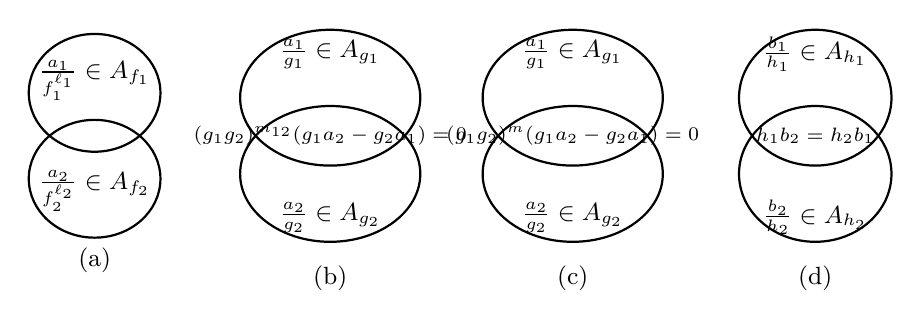
\begin{tikzpicture}[scale=0.88,every node/.style={font=\small}]
  \begin{scope}[shift={(0,0)}]
    \draw[thick] (0,0.62) ellipse (0.95 and 0.85);
    \draw[thick] (0,-0.62) ellipse (0.95 and 0.85);
    \node at (0,0.80) {$\frac{a_1}{f_1^{\ell_1}}\in A_{f_1}$};
    \node at (0,-0.80) {$\frac{a_2}{f_2^{\ell_2}}\in A_{f_2}$};
    \node at (0,-1.80) {(a)};
  \end{scope}
  \begin{scope}[shift={(3.4,0)}]
    \draw[thick] (0,0.55) ellipse (1.30 and 0.98);
    \draw[thick] (0,-0.55) ellipse (1.30 and 0.98);
    \node at (0,1.18) {$\frac{a_1}{g_1}\in A_{g_1}$};
    \node at (0,-1.18) {$\frac{a_2}{g_2}\in A_{g_2}$};
    \node at (0,0) {\scriptsize$(g_1g_2)^{m_{12}}(g_1a_2-g_2a_1)=0$};
    \node at (0,-2.05) {(b)};
  \end{scope}
  \begin{scope}[shift={(6.9,0)}]
    \draw[thick] (0,0.55) ellipse (1.30 and 0.98);
    \draw[thick] (0,-0.55) ellipse (1.30 and 0.98);
    \node at (0,1.18) {$\frac{a_1}{g_1}\in A_{g_1}$};
    \node at (0,-1.18) {$\frac{a_2}{g_2}\in A_{g_2}$};
    \node at (0,0) {\scriptsize$(g_1g_2)^{m}(g_1a_2-g_2a_1)=0$};
    \node at (0,-2.05) {(c)};
  \end{scope}
  \begin{scope}[shift={(10.4,0)}]
    \draw[thick] (0,0.55) ellipse (1.10 and 0.98);
    \draw[thick] (0,-0.55) ellipse (1.10 and 0.98);
    \node at (0,1.18) {$\frac{b_1}{h_1}\in A_{h_1}$};
    \node at (0,-1.18) {$\frac{b_2}{h_2}\in A_{h_2}$};
    \node at (0,0) {\scriptsize$h_1b_2=h_2b_1$};
    \node at (0,-2.05) {(d)};
  \end{scope}
\end{tikzpicture}
\caption{\trStructureSheaf{}的\trBase\trGluability{}。（依原书手绘图重绘。）}\label{fig:base-gluability}
\end{figure}

$a_i/g_i$ 与 $a_j/g_j$ 「在重叠上一致」（即在 $A_{g_i g_j}$ 中一致）意味着：对某个 $m_{ij}$，
\[
(g_ig_j)^{m_{ij}}(g_ja_i-g_ia_j)=0
\]
在 $A$ 中成立。取 $m=\max m_{ij}$（这里我们用到了 $I$ 的有限性），便可统一记号：
\[
(g_ig_j)^{m}(g_ja_i-g_ia_j)=0
\]
对一切 $i$, $j$ 成立（图~\ref{fig:base-gluability}(c)）。令 $b_i=a_ig_i^{m}$（对一切 $i$），并令 $h_i=g_i^{m+1}$（于是 $D(h_i)=D(g_i)$）。这样还能把记号简化得更彻底（图~\ref{fig:base-gluability}(d)）：在每个 $D(h_i)$ 上我们有函数 $b_i/h_i$，而重叠条件就是
\begin{equation*}\tag{4.1.3.2}\label{eq:overlap-condition-simplified}
h_jb_i=h_ib_j.
\end{equation*}
现在 $\bigcup_i D(h_i)=\Spec A$，由此知对某组 $r_i\in A$ 有 $1=\sum_{i=1}^{n}r_ih_i$。定义
\begin{equation*}\tag{4.1.3.3}\label{eq:r-gluing-definition}
r=\sum r_ib_i.
\end{equation*}
这个 $r$ 将就是那个限制到每个 $b_i/h_i$ 上的 $A$ 中元素。的确，由重叠条件 \eqref{eq:overlap-condition-simplified}，
\[
rh_j=\sum_i r_ib_ih_j=\sum_i r_ih_ib_j=b_j.
\]

接下来处理 $I$ 为无穷的情形：选取有限子集 $\{1,\dots,n\}\subset I$，使得 $(f_1,\dots,f_n)=A$（或者等价地，利用 $\Spec A$ 的\trQuasicompactness{}来选取 $D(f_i)$ 的一个有限子覆盖）。利用 \eqref{eq:r-gluing-definition}，如上构造 $r$。我们将证明：对任意 $z\in I-\{1,\dots,n\}$，$r$ 都限制到 $A_{f_z}$ 中我们想要的那个元素 $a_z/f_z^{\ell_z}$ 上。把上面的整个流程用 $\{1,\dots,n,z\}$ 代替 $\{1,\dots,n\}$ 再重演一遍，得到 $r'\in A$，它限制到 $a_i/f_i^{\ell_i}$（对 $i\in\{1,\dots,n,z\}$）。于是由\trBase\trIdentityAxiom，$r'=r$。（注意：我们是在用\trBase{}恒等来\emph{证明}\trBase\trGluability。这正是一个例证，说明恒等公理在某种意义上比可粘性公理更「在先」。）因此，$r$ 限制到 $A_{f_z}$ 中我们想要的那个元素 $a_z/f_z^{\ell_z}$ 上。

\begin{exercise}\label{ex:base-gluability-distinguished-open}
对上述论证作适当改动，证明\trBase\trGluability{}对任意\trDistinguishedOpen{} $D(f)$ 成立。
\end{exercise}

至此，\cref{thm:sheaf-on-distinguished-base}的证明便告完成。\hfill$\square$

\vkthmsync{4}
\begin{remark}[\hard\hard]\label{thm:sections-not-localization}
\cref{thm:structure-sheaf-definition}与\cref{thm:sheaf-on-distinguished-base}暗示了一种可能相当利落的办法，来描述 $\OO_{\Spec A}$ 在\emph{任意}\trOpenSubset{}上的\trSection：或许 $\OO_{\Spec A}(U)$ 就是 $A$ 在「在 $U$ 的任何一点处都不消失的函数全体」这个\trMultiplicativeSubset{}上的\trLocalization？这并不成立。一个反例（日后你将能使它精确化）：设 $\Spec A$ 为两份 $\mathbb{A}^2_k$ 沿其原点粘合所得的空间（显式方程见 (24.3.8.1)），并令 $U$ 为（诸）原点的补集。那么，在第一份 $\mathbb{A}^2_k\smallsetminus\{(0,0)\}$ 上取值 $1$、在第二份 $\mathbb{A}^2_k\smallsetminus\{(0,0)\}$ 上取值 $0$ 的那个函数，就不是这种形式。（追问：若粘合的是沿一点相贴的两份 $\mathbb{A}^1_k$，这套讨论为何就行不通了？）
\end{remark}

\textbf{4.1.5.\ 供日后使用的重要观念：由 $A$-模而来的 $\OO_{\Spec A}$-模。}\quad \cref{thm:sheaf-on-distinguished-base}的下面这个推广，对第~6~章中\trQCSheaf{}的定义将是必不可少的。你可以把这些练习留到那时再做，但趁这些想法在你脑海里还新鲜，现在就做也许最容易。

\begin{exercise}[重要练习兼定义]\label{ex:module-sheaf-on-base}
设 $M$ 是一个 $A$-\trModule。证明：下面的构造给出\trDistinguishedBase{}上的一个\trSheaf{} $\widetilde{M}$。定义 $\widetilde{M}(D(f))$ 为 $M$ 在「在 $V(f)$ 之外不消失的函数全体」这个\trMultiplicativeSubset{}上的\trLocalization；并照 $\OO_{\Spec A}$ 的情形完全类似地定义诸\trRestrictionMap{} $\mathrm{res}_{D(f),D(g)}$。证明这给出\trDistinguishedBase{}上的一个\trSheaf，从而给出 $\Spec A$ 上的一个\trSheaf。再证明这是一个 $\OO_{\Spec A}$-\trModule。
\end{exercise}

\vkthmsync{6}
\begin{remark}[重要注记]\label{thm:module-equalizer-exactness}
在解答上一练习的过程中，你将证明：若 $(f_i)_{i\in I}=A$，则
\begin{equation*}\tag{4.1.6.1}\label{eq:module-equalizer-sequence}
0\longrightarrow M\longrightarrow\prod_{i\in I}M_{f_i}\longrightarrow\prod_{i\neq j\in I}M_{f_i f_j}
\end{equation*}
（对照 \eqref{eq:equalizer-structure-sheaf}）是正合的。特别地，$M$ 可以等同于 $M_{f_1}\times\cdots\times M_{f_r}$ 的一个具体的\trSubmodule。尽管对每个 $f_i$ 而言 $M\to M_{f_i}$ 未必是\trInclusionMap，但 $M\to M_{f_1}\times\cdots\times M_{f_r}$ \emph{确实}是\trInclusionMap。这一点日后会派上用场：我们会想证明「若 $M$ 具有某条好性质，则 $M_f$ 也有」，那将很容易；我们还会想证明另一方向的推理：若 $(f_1,\dots,f_n)=A$ 且诸 $M_{f_i}$ 都有这条性质，则 $M$ 也有。这个想法将在\trAffineCommunicationLemma{}~5.3.2（Affine Communication Lemma）中得到精确表述。
\end{remark}

\begin{exercise}\label{ex:stalk-tilde-m-localization}
设 $\mathfrak{p}$ 是 $A$ 的一个\trPrimeIdeal。描述一个\trCanonical\trIsomorphism{} $\widetilde{M}_{[\mathfrak{p}]}\tilde{\longrightarrow}M_{\mathfrak{p}}$，它联系 $\widetilde{M}$ 的\trStalk{}与 $M$ 的\trLocalization。特别地，$\OO_{\Spec A}$ 在点 $[\mathfrak{p}]$ 处的\trStalk{}就是\trLocalRing{} $A_{\mathfrak{p}}$。
\end{exercise}

下面这条练习展示：一条重要的结论，从代数与几何两种视角去看，理解方式可以何等不同。

\begin{exercise}\label{ex:module-to-product-localizations}
设 $M$ 是一个 $A$-\trModule。证明自然映射
\[
M\lhook\joinrel\longrightarrow\prod_{\mathfrak{p}\in\Spec A}M_{\mathfrak{p}}
\]
是\trInjectiveMap，且有两种证法：(a)~考虑该映射的\trKernel，证明其中任何元素必为 $0$；(b)~把\cref{ex:sections-determined-by-germs}（\trSheaf{}的\trSection{}由\trGerm{}确定）应用到层 $\widetilde{M}$ 上。（于是：一个 $A$-\trModule{}是零，当且仅当它在所有\trPrimeIdeal{}处的\trLocalization{}都是零；而且我们看到，这同时是 (a)~一条代数事实与 (b)~一条几何事实。）
\end{exercise}

\begin{exercise}\label{ex:module-maps-sheaf-maps}
描述 $A$-\trModule{}之间的映射 $M\to N$ 与 $\OO_{\Spec A}$-\trModule{}之间的映射 $\widetilde{M}\to\widetilde{N}$ 之间的一个\trBijection。（换一种花哨的「翻译」：你这就把 $\catMod{A}$ 描述成了 $\catMod{\OO_{\Spec A}}$ 的一个\trFullSubcategory。）
\end{exercise}

\vkthmsync{7}
\begin{definition}[模的支撑]\label{thm:support-of-module}
受\cref{ex:stalk-tilde-m-localization}与「\trSheaf{}之\trSection{}的\trSupport{}」这一观念（\cref{thm:support-of-section}）的启发，定义 $\mathrm{m}\in M$ 的\textbf{\trSupport}为
\[
\Supp\mathrm{m}:=\{[\mathfrak{p}]\in\Spec A\ :\ \mathrm{m}_{\mathfrak{p}}\neq 0\}\subset\Spec A,
\]
即把 $\mathrm{m}$ 看作 $\widetilde{M}$ 的\trSection{}时的\trSupport。据\cref{ex:support-of-section-closed}，$\Supp\mathrm{m}$ 是 $\Spec A$ 的一个\trClosedSubset。
类似地（仿照\cref{thm:support-of-sheaf}），定义 $M$ 的\textbf{\trSupport}为
\[
\Supp M:=\Supp\widetilde{M}=\{[\mathfrak{p}]\in\Spec A\ :\ M_{\mathfrak{p}}\neq 0\}\subset\Spec A.
\]
这些观念将反复登场。我们将在 \S6.6.3 中更详细地讨论支撑。
\end{definition}

\textbf{4.1.8.\ 反复登场的（反）例。}\quad 「两张平面交于一点」这个例子（\S4.1.4）将作为例子或反例出现许多次。在脑海中常备这样一些例子（或反例）是重要的：它们是「边界标记」，提醒你什么是合理的，以及当你听到一条新命题时应当提防什么。下面这些例子的每次登场都列于索引之中（归在「反复登场的（反）例」名下），因此你能查到它们出现的频率与位置。其中许多条目你眼下还没有语言去理解，但日后可以回到这份清单。
\begin{itemize}
\item 在一点相交的两张平面
\item 仿射空间挖去原点，及其向仿射空间中的\trInclusionMap
\item 原点加倍了的仿射空间
\item \trQuadricSurface{}（及其上的\trCone），$A=k[w,x,y,z]/(wz-xy)$
\item 一条直线上的一个\textbf{\trEmbeddedPoint{}}（embedded point），$k[x,y]/(y^2,xy)$
\item \trProjective{}平面中的 $x^2=0$
\item 概形的无穷\trDisjointUnion{}（尤其是 $\bigsqcup\Spec k[x]/(x^n)$）
\item 态射 $\Spec\overline{\mathbb{Q}}\to\Spec\mathbb{Q}$
\item $k(x)\otimes_k k(y)$
\item $\prod^{\infty}\mathbb{F}_2$
\end{itemize}


\section{概形可视化：幂零元}

\epigraph
  {隐喻的代价，是永远的警惕。}
  {——A.~Rosenbluth 与 N.~Wiener（[Lew, p.~4] 如此归名）}

在 \S3.3 中，我们讨论了如何把\trScheme{}的\trUnderlyingSet{}可视化：在我们先前
关于「传统的点」（即\trClosedPoint）的直观之上添入了\trGenericPoint。其后关于%
\trZariskiTopology{}的讨论与这幅图景吻合得很好。在我们对「\trAffineScheme{}」%
$(\Spec A,\,\OO_{\Spec A})$ 的定义中，还多出了\trNilpotent{}元所携带的一份附加
信息，它们在点的层面上不可见（\S3.2.12），于是现在我们就来弄清如何把它们画出来。
一旦适当的定义就位，我们随即就能把它们粘合起来，画出一般的\trScheme{}的图画。
既然我们是在搭建直观，便不可能做到严格或精确。

作为动机，注意我们有下面这些反转包含关系的双射：
\[
\begin{array}{lcl@{\qquad\qquad}l}
\text{$A$ 的\trMaximalIdeal} & \longleftrightarrow &
  \text{$\Spec A$ 的\trClosedPoint，} &
  \text{（\cref{ex:closed-points-maximal-ideals}）}\\[12pt]
\text{$A$ 的\trPrimeIdeal} & \longleftrightarrow &
  \text{$\Spec A$ 的\trIrreducible{}\trClosedSubset，} &
  \text{（\cref{ex:irreducible-prime-bijection}）}\\[12pt]
\text{$A$ 的\trRadicalIdeal} & \longleftrightarrow &
  \text{$\Spec A$ 的\trClosedSubset。} &
  \text{（\cref{thm:closed-subsets-radical-ideals}）}
\end{array}
\]
若把右边一栏的东西当作「图画」，我们的目标便是弄明白：如何为那些非根的%
\trIdeal{}作画：
\[
\text{$A$ 的\trIdeal} \longleftrightarrow \text{？？？}
\]
（日后我们会以另一种方式把此处严格补全，即引入\emph{\trClosedSubscheme{}}（closed
subscheme）的概念——\trClosedSubset{}的「概形论」版本，见 \S9.1。但我们眼下的
目标只是造出一幅图画。）

作为动机，当我们见到 $\Spec \mathbb{C}[x]/\bigl(x(x-1)(x-2)\bigr)$ 这个表达式时，
会立刻把它解读为 $\mathbb{A}^1_{\mathbb{C}}$ 的一个\trClosedSubset，即
$\{0,\,1,\,2\}$。特别地，映射
$\mathbb{C}[x]\to\mathbb{C}[x]/\bigl(x(x-1)(x-2)\bigr)$ 可以（经中国剩余定理）
解读为：取 $\mathbb{A}^1$ 上的一个函数，并把它限制到三个点 $0$、$1$ 与 $2$ 上。

这将指引我们如何将一个非根\trIdeal{}可视化。最简单的例子是
$\Spec \mathbb{C}[x]/(x^2)$（\cref{ex:small-schemes-dual-numbers}(a)）。作为
$\mathbb{A}^1$ 的子集，它恰是原点 $0=[(x)]$——我们习惯把它想成
$\Spec \mathbb{C}[x]/(x)$（即对应于\trIdeal{} $(x)$，而非 $(x^2)$）。我们想以
某种方式丰富这幅图画。我们应当依据「商记住了哪些信息」来画
$\mathbb{C}[x]/(x^2)$：多项式 $f(x)$ 的\trImage，就是「它在 $0$ 处的值」与「它的导数」
这一信息（参看\cref{ex:derivatives-dual-numbers}）。于是我们把它画成那个点、
再多上一点点——点上的一点无穷小「\trFuzz{}」（fuzz）（见图~\ref{fig:quotients-of-cx}）。
限制序列 $\mathbb{C}[x]\to\mathbb{C}[x]/(x^2)\to\mathbb{C}[x]/(x)$ 应当被解读为
层层嵌套的图画：
\[
\mathbb{C}[x] \twoheadrightarrow \mathbb{C}[x]/(x^2) \twoheadrightarrow \mathbb{C}[x]/(x),
\]
\[
f(x) \longmapsto f(0).
\]
同样，$\mathbb{C}[x]/(x^3)$ 记住的信息还要更多——二阶导数也在其中。于是我们把它
画成带有更多\trFuzz{}的点 $0$。

\begin{figure}[htbp]
\centering
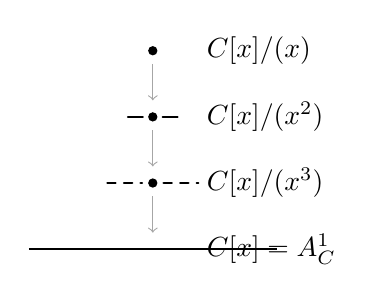
\begin{tikzpicture}[scale=1.05]
  \fill (0,0) circle (1.6pt);
  \node[right=16pt] at (0,0) {$\Spec \mathbb{C}[x]/(x)$};
  \draw[gray!70,->] (0,-0.16) -- (0,-0.60);
  \fill (0,-0.80) circle (1.6pt);
  \draw[thick,line cap=round] (-0.30,-0.80) -- (-0.12,-0.80);
  \draw[thick,line cap=round] (0.12,-0.80) -- (0.30,-0.80);
  \node[right=16pt] at (0,-0.80) {$\Spec \mathbb{C}[x]/(x^2)$};
  \draw[gray!70,->] (0,-0.96) -- (0,-1.40);
  \fill (0,-1.60) circle (1.6pt);
  \draw[thick,dashed,line cap=round] (-0.55,-1.60) -- (-0.13,-1.60);
  \draw[thick,dashed,line cap=round] (0.13,-1.60) -- (0.55,-1.60);
  \node[right=16pt] at (0,-1.60) {$\Spec \mathbb{C}[x]/(x^3)$};
  \draw[gray!70,->] (0,-1.76) -- (0,-2.20);
  \draw[thick] (-1.5,-2.40) -- (1.5,-2.40);
  \node[right=16pt] at (0,-2.40) {$\Spec \mathbb{C}[x]=\mathbb{A}^1_{\mathbb{C}}$};
\end{tikzpicture}
\caption{$\mathbb{C}[x]$ 诸商环的图画。（依原书手绘图重绘。）}%
\label{fig:quotients-of-cx}
\end{figure}

更多的微妙之处出现在二维情形（见图~\ref{fig:quotients-of-cxy}）。考虑
\[
\Spec \mathbb{C}[x,y]/(x,y)^2,
\]
它夹在两个我们十分熟悉的\trRing{}之间：
\[
\mathbb{C}[x,y] \twoheadrightarrow \mathbb{C}[x,y]/(x,y)^2 \twoheadrightarrow \mathbb{C}[x,y]/(x,y),
\]
\[
f(x,y) \longmapsto f(0,0).
\]
同样，对 $(x,y)^2$ 取商记住了「沿一切方向」的一阶导数。我们把它画成围绕该点的%
\trFuzz{}，形状是一个圆（没有任何方向享有特权）。类似地，$(x,y)^3$ 记住了「沿一切
方向」的二阶导数——更大的一圈圆形\trFuzz{}。

\begin{figure}[htbp]
\centering
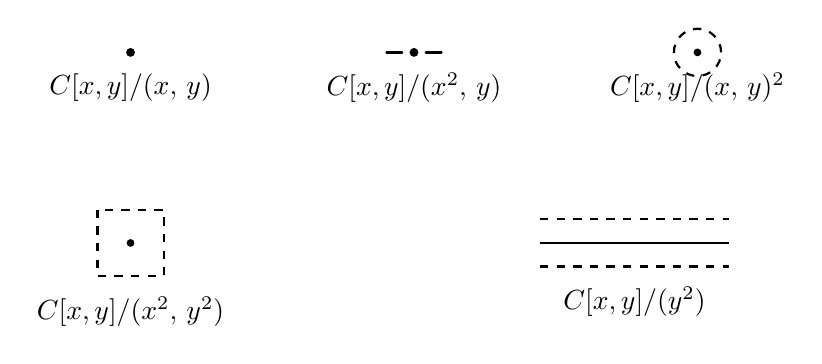
\begin{tikzpicture}[scale=1.0]
  \fill (0,0) circle (1.6pt);
  \node[below=4pt] at (0,0) {$\Spec \mathbb{C}[x,y]/(x,\,y)$};
  \fill (3.6,0) circle (1.6pt);
  \draw[thick,line cap=round] (3.25,0) -- (3.45,0);
  \draw[thick,line cap=round] (3.75,0) -- (3.95,0);
  \node[below=4pt] at (3.6,0) {$\Spec \mathbb{C}[x,y]/(x^2,\,y)$};
  \draw[thick,dashed] (7.2,0) circle (0.30);
  \fill (7.2,0) circle (1.4pt);
  \node[below=4pt] at (7.2,0) {$\Spec \mathbb{C}[x,y]/(x,\,y)^2$};
  \draw[thick,dashed] (-0.42,-2.0) rectangle (0.42,-2.84);
  \fill (0,-2.42) circle (1.4pt);
  \node[below=4pt] at (0,-2.84) {$\Spec \mathbb{C}[x,y]/(x^2,\,y^2)$};
  \draw[thick,dashed] (5.2,-2.12) -- (7.6,-2.12);
  \draw[thick] (5.2,-2.42) -- (7.6,-2.42);
  \draw[thick,dashed] (5.2,-2.72) -- (7.6,-2.72);
  \node[below=4pt] at (6.4,-2.72) {$\Spec \mathbb{C}[x,y]/(y^2)$};
\end{tikzpicture}
\caption{$\mathbb{C}[x,y]$ 诸商环的图画。（依原书手绘图重绘。）}%
\label{fig:quotients-of-cxy}
\end{figure}

换作考虑\trIdeal{} $(x^2,\,y)$。它记住的只是沿 $x$ 方向的导数——给定一个多项式，
我们记住它在 $0$ 处的值，以及 $x$ 的系数。我们画出的\trFuzz{}便只沿 $x$ 方向，以此把
这些信息记住。

至此，我们对给更多这一类东西作画已有了一些抓手，但它如今更像一门艺术，而非一门
科学。比如说，$\Spec \mathbb{C}[x,y]/(x^2,\,y^2)$ 或许可以画成原点四周一块
毛茸茸的正方形。（你能相信这个正方形既内接于圆形\trFuzz{}
$\Spec \mathbb{C}[x,y]/(x,y)^3$、又外接于圆形\trFuzz{}
$\Spec \mathbb{C}[x,y]/(x,y)^2$ 吗？）这个例子的一个特征是：给定一个\trRing{} $A$
（比如 $\mathbb{C}[x,y]$）的两个\trIdeal{} $I$ 与 $J$，你对 $\Spec A/(I,\,J)$
的毛茸茸图画，应当是你关于 $\Spec A/I$ 与 $\Spec A/J$ 在 $\Spec A$ 中的图画
二者的「相交」。（你将在练习~9.1.I(a) 中把这一点弄精确。）比如说，
$\Spec \mathbb{C}[x,y]/(x^2,\,y^2)$ 应当是两条加厚直线之交。（你会如何画
$\Spec \mathbb{C}[x,y]/(x^5,\,y^3)$？$\Spec \mathbb{C}[x,y,z]/(x^3,\,y^4,\,z^5,\,(x+y+z)^2)$？
$\Spec \mathbb{C}[x,y]/\bigl((x,y)^5,\,y^3\bigr)$？）

最后一个例子将在 \S6.6 中激励我们：$\Spec \mathbb{C}[x,y]/(y^2,\,xy)$。知道
$\mathbb{C}[x,y]$ 中的多项式模 $(y^2,\,xy)$ 后是什么，就等价于既知道它在
$x$-轴上的取值，又知道原点附近的一阶微分信息。这值得仔细想透：你能在
图~\ref{fig:nonreduced-y2xy} 中（纵使并不完美地）看出这些信息是如何被捕捉的吗？

\begin{figure}[htbp]
\centering
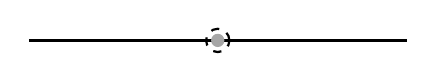
\begin{tikzpicture}[scale=1.0]
  \draw[thick] (-2.4,0) -- (2.4,0);
  \fill[gray!70] (0,0) circle (2.4pt);
  \draw[thick,dashed] (0,0) circle (4.2pt);
\end{tikzpicture}
\caption{$\Spec k[x,y]/(y^2,\,xy)$ 这个\trScheme{}的一幅图。原点处的\trFuzz{}标示出
「非\trReduced{}性」位于何处。（依原书手绘图重绘。）}%
\label{fig:nonreduced-y2xy}
\end{figure}

我们的图画捕捉到了一些你已经对其抱有直观的有用信息。比如说，考虑抛物线
$y=x^2$ 与 $x$-轴（在 $xy$ 平面中）的相交；见图~\ref{fig:scheme-theoretic-intersection}。
你已经有这样的感觉：这个相交的\trMultiplicity{}是 $2$。用这种可视化语言来说，我们把这个交
解读为（在 $\Spec \mathbb{C}[x,y]$ 中的）一次相交：
\begin{align*}
\Spec \mathbb{C}[x,y]/(y-x^2) \cap \Spec \mathbb{C}[x,y]/(y)
  &= \Spec \mathbb{C}[x,y]/(y-x^2,\,y)\\
  &= \Spec \mathbb{C}[x,y]/(y,\,x^2),
\end{align*}
我们把这解读为如下事实：抛物线与这条直线不只是以\trMultiplicity{} $2$ 相遇，而且「\trMultiplicity{} $2$」
这一部分是沿 $x$-轴方向的。你将在练习~9.1.I(b) 中把这个例子弄精确。

\begin{figure}[htbp]
\centering
\begin{tikzpicture}[scale=1.0]
  \draw[thick] plot[domain=-0.75:0.75] (\x,{1.9*\x*\x});
  \node at (2.1,0.55) {相交};
  \draw[thick] (3.2,0.55) -- (4.6,0.55);
  \node at (5.15,0.55) {$=$};
  \draw[line width=2.2pt] (5.9,0.55) -- (6.3,0.55);
\end{tikzpicture}
\caption{抛物线 $y=x^2$ 与 $x$-轴的「概形论」相交是一个非\trReduced{}\trScheme%
（\trFuzz{}沿 $x$ 方向）。（依原书手绘图重绘。）}%
\label{fig:scheme-theoretic-intersection}
\end{figure}

\textbf{4.2.1.}\quad 日后在讨论\trAssociatedPoint{}（associated points）时，我们会把\trFuzz{}的
位置说得更加精确。届时将看到：在合理的情形下，\trFuzz{}集中在\trClosedSubset{}上
（练习~6.6.N）。

\epigraph
  {人们一再地说，几何是在画得糟糕的图形上作良好推理的艺术；然而这些图形若要不
   欺骗我们，就必须满足一定的条件：各部分之间的比例可以被大幅度地改动，但各个
   部分的相对位置却不容搅乱。}
  {——\trn{H.~Poincar\'e}{\trPoincare{}}，[Po1, p.~2]（参看 J.~Stillwell 的英译
   [Po2, p.~ix]）}


\section{\trScheme{}的定义}

\textbf{4.3.1.}\ \emph{\trhDefinition{}。}\quad 现在我们终于可以在一般情形下定义%
\emph{\trScheme}了。首先，定义\textbf{\trRingedSpace{}之间的\trIsomorphism}%
$(X,\OO_X)\to(Y,\OO_Y)$ 为：(i)~一个\trHomeomorphism{} $\pi\colon X\to Y$，以及
(ii)~$\OO_X$ 与 $\OO_Y$ 这两个\trSheaf{}之间的一个\trIsomorphism——这里经 $\pi$ 把
二者视为同一个空间上的\trSheaf。（更确切地说，(ii) 是 $Y$ 上诸\trSheaf{}的一个%
\trIsomorphism{} $\OO_Y\tilde{\longrightarrow}\pi_*\OO_X$；或者等价地，是 $X$ 上诸%
\trSheaf{}的一个\trIsomorphism{} $\pi^{-1}\OO_Y\tilde{\longrightarrow}\OO_X$。）
换言之，我们得到的是「集合、\trTopology{}与\trStructureSheaf」的一种「对应」。每个%
\trIsomorphism{} $\alpha\colon(X,\OO_X)\to(Y,\OO_Y)$ 显然都有一个「逆%
\trIsomorphism{}」$\alpha^{-1}\colon(Y,\OO_Y)\to(X,\OO_X)$。

一个\textbf{\trAffineScheme}，就是对某个 $A$ \trIsomorphic{}于
$(\Spec A,\OO_{\Spec A})$ 的\trRingedSpace。一个\textbf{\trScheme} $(X,\OO_X)$ 是
这样的\trRingedSpace：$X$ 的任何一点都有开\trNeighborhood{} $\mathsf{U}$，使得
$(\mathsf{U},\OO_{X|\mathsf{U}})$ 是一个\trAffineScheme。\trScheme{}上的\trTopology{}
称为\textbf{\trZariskiTopology}。\trScheme{}可以记作 $(X,\OO_X)$，但人们也常把它
记作 $X$，而将\trStructureSheaf{} $\OO_X$ 隐而不写。

\textbf{\trScheme{}之间的\trIsomorphism} $(X,\OO_X)\to(Y,\OO_Y)$ 就是「作为%
\trRingedSpace{}的\trIsomorphism」。回想 \S2.2.2 中 $\Gamma(\cdot,\cdot)$ 的定义。
若 $\mathsf{U}\subset X$ 是一个\trOpenSubset，则 $\Gamma(\mathsf{U},\OO_X)$ 的元素
便称为\textbf{$\mathsf{U}$ 上的函数}；这推广了\trAffineScheme{}上函数的定义
（\S3.2.1）。

\textbf{4.3.2.}\ \emph{\trhRemark{}。}\quad 从\trAffineScheme{}上\trStructureSheaf{}
的定义出发，有几件事是一目了然的。首先，若有人告知我们 $(X,\OO_X)$ 是一个%
\trAffineScheme，我们便可以取\trGlobalSections{}所成之\trRing{}来复原它的\trRing
（亦即找出使 $\Spec A=X$ 的那个\trRing{} $A$），因为 $X=D(1)$，于是：
\begin{align*}
\Gamma(X,\OO_X)&=\Gamma(D(1),\OO_{\Spec A}) &&\text{由于 }D(1)=\Spec A\\
&=A.
\end{align*}
（你可以核验：我们实际得到的还要更多，而且能够「把 $X$ 认作\trScheme{} $\Spec A$」：
我们会
得到一个\trIsomorphism{}
$\pi\colon(\Spec\Gamma(X,\OO_X),\,\OO_{\Spec\Gamma(X,\OO_X)})
\tilde{\longrightarrow}(X,\OO_X)$。例如，若 $\mathfrak{m}$ 是
$\Gamma(X,\OO_X)$ 的一个\trMaximalIdeal，则 $\{\pi([\mathfrak{m}])\}=V(\mathfrak{m})$。）
下一道练习将把这些想法严格化——它们比乍看之下更微妙。

\textbf{4.3.3.}\ \emph{\trhCaveat{}。}\quad 定义并未把「两个\textbf{\trAffine%
\trOpenSubset}（affine open subset）的交仍是\trAffine{}的」包含在内（反例见%
\mbox{练习~4.4.C}），尽管在大多数令人感兴趣的场合，这一点确实成立（见%
\mbox{命题~11.2.13}）。

\begin{exercise}[富于启发的练习（可能怪异地令人困惑）]\label{ex:scheme-isos-ring-isos}
描述诸\trIsomorphism{} $\Spec A\tilde{\longrightarrow}\Spec A'$（视之为%
\trRingedSpace{}之间的\trIsomorphism）与诸\trRing{}\trIsomorphism{}
$A'\tilde{\longrightarrow}A$ 之间的一个\trBijection。提示：最难的部分是证明：若%
\trIsomorphism{} $\pi\colon\Spec A\tilde{\longrightarrow}\Spec A'$ 诱导出一个%
\trIsomorphism{} $\pi^{\sharp}\colon A'\tilde{\longrightarrow}A$，而后者又诱导出%
\trIsomorphism{} $\rho\colon\Spec A\tilde{\longrightarrow}\Spec A'$，则 $\pi=\rho$。
先在点的层面上证明它；这（出人意料地）恰是最棘手之处。然后证明：作为%
\trTopologicalSpace{}之间的映射有 $\pi=\rho$。最后，为在\trStructureSheaf{}的层面上
证明 $\pi=\rho$，请动用\trDistinguishedBase。尽管随意使用本节后文给出的洞见，但要
小心避免循环论证。即便你在这道练习上苦苦挣扎而失败（直到读了后面几节之前），也会
有所裨益。
\end{exercise}

更一般地，给定 $f\in A$，有 $\Gamma(D(f),\OO_{\Spec A})\cong A_f$。于是，在集合的
自然\trInclusionMap{} $\Spec A_f\hookrightarrow\Spec A$ 之下，$\Spec A$ 上的%
\trZariskiTopology{}限制后给出的正是 $\Spec A_f$ 上的\trZariskiTopology
（\cref{ex:subspace-topology-inclusions}），而 $\Spec A$ 的\trStructureSheaf{}也
限制为 $\Spec A_f$ 的\trStructureSheaf，下一道练习将表明这一点。

\begin{exercise}[重要而容易的练习]\label{ex:distinguished-open-ringed-space-iso}
设 $f\in A$。证明：在把 $\Spec A$ 中的 $D(f)$ 认同于 $\Spec A_f$ 之时（\S3.5），
存在\trRingedSpace{}之间的一个自然\trIsomorphism
\[
(D(f),\OO_{\Spec A}|_{D(f)})\;\tilde{\longleftrightarrow}\;(\Spec A_f,\OO_{\Spec A_f}).
\]
提示：注意 $\Spec A_f$ 的诸\trDistinguishedOpen{}
本来就是 $\Spec A$ 中的\trDistinguishedOpen。
\end{exercise}

\begin{exercise}[容易的练习]\label{ex:open-subset-of-scheme}
若 $X$ 是一个\trScheme，而 $\mathsf{U}$ 是\emph{任意}一个\trOpenSubset，证明
$(\mathsf{U},\OO_{X|\mathsf{U}})$ 也是一个\trScheme。
\end{exercise}

\textbf{4.3.4.}\ \emph{\trhDefinition{}。}\quad 我们称 $(\mathsf{U},\OO_{X|\mathsf{U}})$
为 $X$ 的一个\textbf{\trOpenSubscheme}（open subscheme）。若 $\mathsf{U}$ 还是一个%
\trAffineScheme，我们常说 $\mathsf{U}$ 是一个\textbf{\trAffine\trOpenSubset}，或一个%
\textbf{\trAffine\trOpenSubscheme}（affine open subscheme），或者有时非正式地，就径称
一个\textbf{\trAffine{}开}（affine open）。例如，$D(f)$ 就是 $\Spec A$ 的一个%
\trAffine\trOpenSubscheme。（趣闻：「$\Spec A$ 的每个\trAffine\trOpenSubscheme{}都
形如 $D(f)$」并不成立；例子见 \S19.11.10。）

\begin{exercise}[容易的练习]\label{ex:affine-opens-base}
证明：若 $X$ 是一个\trScheme，则诸\trAffine\trOpenSet{}构成\trZariskiTopology{}的
一组\trBase。
\end{exercise}

\begin{exercise}[容易的练习]\label{ex:disjoint-union-schemes}
\textbf{\trScheme{}的\trDisjointUnion}按你期望的方式定义：它就是集合的%
\trDisjointUnion，配上你所期望的\trTopology（于是它就是\trTopologicalSpace{}的%
\trDisjointUnion），再配上你所期望的\trSheaf。我们用符号 $X\sqcup Y$ 表示 $X$ 与
$Y$ 的\trDisjointUnion，
因为一旦我们知道了「\trScheme{}的\trMorphism」为何物，这个构造就会被证实是\trScheme{}
的\trCategory{}中的\trCoproduct（\mbox{练习~7.3.K}）。

(a)~证明：\emph{有限}多个\trAffineScheme{}的\trDisjointUnion{}也是一个%
\trAffineScheme。（提示：\cref{ex:product-ring-homeomorphism}。）

(b)~（\emph{非\trAffineScheme{}的第一个例子}）证明：无穷多个（非空）%
\trAffineScheme{}的\trDisjointUnion{}不是一个\trAffineScheme。（提示：%
\trAffineScheme{}都是\trQuasicompact{}的，见\cref{ex:spec-quasicompact}(a)。这基本
上已在注记~3.6.6 中作答。）
\end{exercise}

\textbf{4.3.5.}\ \emph{\trhRemark{}：初窥\trClosedSubscheme{}。}\quad \trScheme{}的%
\trOpenSubset{}自带一种自然的\trScheme{}结构（定义~4.3.4）。作为对照，%
\trClosedSubset{}却可以带有许多种「自然」的\trScheme{}结构。我们稍后将讨论此事
（\S9.1），但眼下你只需知道：$X$ 的一个\trClosedSubscheme，非正式地说，就是 $X$ 的
某个\trClosedSubset{}上的一种特殊的\trScheme{}结构。举个例子：若 $I\subset A$ 是
一个\trIdeal，则 $\Spec A/I$ 就赋予\trClosedSubset{} $V(I)\subset\Spec A$ 一种%
\trScheme{}结构；但要注意，具有同一\trVanishingSet{}的\trIdeal{}可以不止一个
（例如 $k[x]$ 中的 $(x)$ 与 $(x^2)$）。

\textbf{4.3.6.\ \trStructureSheaf{}的诸\trStalk{}：\trGerm{}、在一点处的取值，以及
一点的\trResidueField{}。}\quad 与一切\trSheaf{}一样，\trStructureSheaf{}也有诸%
\trStalk；而且毫不意外，从代数的视角看，它们饶有趣味。事实上，我们此前早已见过它们。

\textbf{4.3.7.}\ \emph{\trhDefinition{}。}\quad 若一个\trRingedSpace{}的诸\trStalk{}
都是\trLocalRing，就称它是一个\textbf{\trLocallyRingedSpace{}}。由%
\cref{ex:stalk-tilde-m-localization}，$\OO_{\Spec A}$ 在点 $[\mathfrak{p}]$ 处的%
\trStalk{}就是\trLocalRing{} $A_{\mathfrak{p}}$。

于是，\trScheme{}都是\trLocallyRingedSpace{}。而\trManifold{}则是\trLocally%
\trRingedSpace{}的另一个例子；见 \S2.1.1。在这两种情形，对\trMaximalIdeal{}取商都
可以理解为「在一点处取值」。\trLocalRing{} $\OO_{X,p}$ 的\trMaximalIdeal{}记作
$\mathfrak{m}_{X,p}$ 或 $\mathfrak{m}_p$，而\trResidueField{}
$\OO_{X,p}/\mathfrak{m}_p$ 记作 $\kappa(p)$。\trLocallyRingedSpace{} $X$ 的%
\trOpenSubset{} $\mathsf{U}$ 上的每个函数 $f$，在 $\mathsf{U}$ 的每一点 $p$ 处都有
一个值：\textbf{$f$ 在 $p$ 处的值}（记作 $f(p)$）是 $f$ 在 $p$ 处的\trGerm{}在%
\trCanonical{}映射 $\OO_{X,p}\to\kappa(p)$ 之下的像。若一个函数在点 $p$ 处的值为
$0$，就称它在点 $p$ 处\textbf{为零}。（这推广了 \S3.2.1 中定义的「函数在 $\Spec A$
上取值」的观念。）请注意：在一般的\trRingedSpace{}上，甚至连「函数为零」这个说法都
无法赋以意义。

\begin{exercise}[有用练习]\label{ex:vanishing-locus-closed}
(a)~设 $f$ 是\trLocallyRingedSpace{} $X$ 上的一个函数，证明：$X$ 中使 $f$ 为零的
点构成的子集是闭的。提示：设 $f$ 是\trRingedSpace{} $X$ 上的一个函数，证明：$X$ 中
使 $f$ 的\trGerm{}为\trInvertible{}的点构成的子集是开的。（于是，在%
\trLocallyRingedSpace{}上，函数取非零\emph{值}的\trLocus{}是开的；与之相对，
函数取非零\trGerm{}的\trLocus{}则是闭的，见\cref{thm:caution-value-vs-germ}。）

(b)~证明：若 $f$ 是\trLocallyRingedSpace{}上一个无处为零的函数，则 $f$ 是%
\trInvertible{}的。
\end{exercise}

考虑\trAffineScheme{} $\Spec A$ 的一点 $[\mathfrak{p}]$。（当然，\trScheme{}的任何
一点都可以这样看待，因为每一点都有\trAffine{}开\trNeighborhood。）$[\mathfrak{p}]$
处的\trResidueField{}是 $A_{\mathfrak{p}}/\mathfrak{p}A_{\mathfrak{p}}$，它%
\trIsomorphic{}于 $\mathrm{K}(A/\mathfrak{p})$，即该\trQuotient{}的\trFractionField。
值得注意的是：在
$\mathfrak{p}$ 处\trLocalization{}与对 $\mathfrak{p}$ 取商二者「交换」，也就是说，
下图交换。
\begin{equation*}\tag{4.3.7.1}\label{eq:localize-quotient-diagram}
\begin{tikzcd}[row sep=2.6em, column sep=4em]
 & A_{\mathfrak{p}} \ar[dr, "\text{取商}"'] & \\
A \ar[ur, "\text{局部化}"] \ar[dr, "\text{取商}"'] & &
A_{\mathfrak{p}}/\mathfrak{p}A_{\mathfrak{p}}\ =\ \mathrm{K}(A/\mathfrak{p}) \\
 & A/\mathfrak{p} \ar[ur, "\text{局部化（即 }\mathrm{K}(\cdot)\text{）}"'] &
\end{tikzcd}
\end{equation*}

例如，考虑\trScheme{} $\mathbb{A}^2_k=\Spec k[x,y]$，其中 $k$ 是\trCharacteristic{}
不为 $2$ 的一个\trField。则 $(x^2+y^2)/x(y^2-x^5)$ 在 $y$-轴与\trCurve{}
$y^2-x^5$ 之外
是一个函数。它在 $(2,4)$ 处的值（这么说意指 $[(x-2,\,y-4)]$）是
$(2^2+4^2)/(2(4^2-2^5))$，即
\[
\frac{x^2+y^2}{x(y^2-x^5)}\equiv\frac{2^2+4^2}{2(4^2-2^5)}
\]
在\trResidueField{}中成立——若你觉得神秘，不妨核验一番。而它在 $[(y)]$——$x$-轴的%
\trGenericPoint——处的值是 $-x^2/x^6=-1/x^4$，这只需令 $y$ 为 $0$ 便可看出。这确实是
$k[x,y]/(y)$ 的\trFractionField，即 $k(x)$ 中的一个元素。（如果你自认为只关心%
\trAlgClosedField，那就让这个例子给你敲响第一声警钟：一般地，
$A_{\mathfrak{p}}/\mathfrak{p}A_{\mathfrak{p}}$ 未必是\trAlgClosed{}的，哪怕 $A$ 是
有限生成的 $\mathbb{C}$-代数！）

如果有什么让你心里没底，你就该自己编一个例子来宽宽心。这里就有一个：$27/4$ 是
$\Spec\mathbb{Z}\smallsetminus\{[(2)],\,[(7)]\}$ 上的一个函数——其实在一个还要更大
的\trOpenSubset{}上亦是如此。它在 $[(5)]$ 处的值是多少？答：$2/(-1)\equiv-2
\pmod{5}$。它在\trGenericPoint{} $[(0)]$ 处的值是多少？答：$27/4$。它在何处为零？
在 $[(3)]$ 处。

\textbf{4.3.8.}\ \emph{\trhDefinition{}：$\OO_X$-\trModule{}在一点处的\trFiber{}与%
\trRank{}。}\quad 设 $\scr{F}$ 是\trScheme{} $X$ 上的一个 $\OO_X$-\trModule（或者
更一般地，是某个\trLocallyRingedSpace{}上的），定义 $\scr{F}$ 在点 $p\in X$ 处的%
\textbf{\trFiber}（fiber）为
\[
\scr{F}|_p:=\scr{F}_p\otimes_{\OO_{X,p}}\kappa(p).
\]
这个\trFiber{}是 $\kappa(p)$ 上的一个\trVectorSpace。该\trVectorSpace{}的%
\trDimension{} $\dim_{\kappa(p)}\scr{F}|_p$ 称为\textbf{$\scr{F}$ 在 $p$ 处的%
\trRank}（rank），记作 $\mathrm{rank}_p\,\scr{F}$。例如，$\OO_X|_p$ 就是
$\kappa(p)$，而
$\mathrm{rank}_p\,\OO_X=1$。

\textbf{4.3.9.}\ \hard\ \emph{\trhDefinition{}：形形色色的\trManifold{}。}\quad 用
同样的办法，我们也能干净利落、简洁明了地定义（种种不同观念下的）\trManifold。一个%
\textbf{\trTopology}（相应地，\textbf{\trDifferentiable}、
$C^\infty$＝\textbf{\trSmooth}）的（\trReal）\textbf{\trManifold}，是一个%
\trRingedSpace{} $(X,\OO_X)$：其底\trTopologicalSpace{} $X$ 是\trHausdorff{}的、%
\trSecondCountable{}的，并且 $X$ 的任何一点都有开\trNeighborhood{} $\mathsf{U}$，
使得 $(\mathsf{U},\OO_{X|\mathsf{U}})$ \trIsomorphic{}于「$\mathbb{R}^n$ 中的一个%
\trOpenBall，连同其上的\trContinuous（相应地，\trDifferentiable、
$C^\infty$＝\trSmooth）\trRealValued{}函数之\trSheaf」。不带修饰语的单说
「\trManifold」，常指的就是\textbf{光滑\trManifold}。一个%
\textbf{\trComplex\trManifold}则是一个\trRingedSpace{} $(X,\OO_X)$：其底%
\trTopologicalSpace{} $X$ 是\trHausdorff{}的、\trSecondCountable{}的，并且 $X$ 的
任何一点都有开\trNeighborhood{} $\mathsf{U}$，使得 $(\mathsf{U},\OO_{X|\mathsf{U}})$
\trIsomorphic{}于「$\mathbb{C}^n$ 中的一个\trOpenBall，连同其上的%
\trHolomorphic{}函数之\trSheaf」。


\section{三个例子}

我们现在给出三个篇幅较长的例子。短期目标是看到：我们确实能够驾驭\trStructureSheaf，并能对有趣的%
\trOpenSet{}算出其\trSection{}环——这些\trOpenSet{}不再只是\trAffineScheme{}的\trDistinguishedOpen。%
长期目标是遇见一些有趣的例子，它们将在日后反复登场。

\textbf{4.4.1.\ 第一个例子：挖去原点的（\trAffine）平面。}\quad 这个例子将让你看到：\trDistinguishedBase{}%
是一种你真正能够上手的东西。设 $A=k[x,y]$，于是 $\Spec A=\mathbb{A}^2_k$。我们来把\trOpenSet{}%
$U=\mathbb{A}^2\smallsetminus\{(0,0)\}=\mathbb{A}^2\smallsetminus\{[(x,y)]\}$ 上的函数空间算出来。

这是不是一个\trDistinguishedOpen，并非一目了然。（事实上它不是——哪怕你现在还看不出来，%
再过几段你多半就能想明白缘由。仅证明 $(x,y)$ 不是\trPrincipalIdeal{}是不够的。）但无论如何，我们可以把它%
描述为两个\emph{确实}是\trDistinguishedOpen{}的东西之并：$U=D(x)\cup D(y)$。我们将把 $D(x)$ 上的%
函数与 $D(y)$ 上的函数粘合起来，从而找出 $U$ 上的函数。

根据\cref{thm:structure-sheaf-definition}，$D(x)$ 上的函数是 $A_x=k[x,y,1/x]$；$D(y)$ 上的函数是%
$A_y=k[x,y,1/y]$。注意：$A$ \trInjectiveMap{}到它的诸\trLocalization{}之中（只要不让 $0$ 被取逆），%
因为它是\trIntegralDomain（\cref{ex:when-localization-is-injective}）；于是 $A$ \trInjectiveMap{}入%
$A_x$ 与 $A_y$ 二者，而这两者又都\trInjectiveMap{}入 $A_{xy}$（而且确实\trInjectiveMap{}入%
$k(x,y)=K(A)$）。于是，我们要找的是 $D(x)$ 与 $D(y)$ 上在 $D(x)\cap D(y)=D(xy)$ 处相互一致的%
函数；换言之，我们是在 $A_{xy}$（或在 $k(x,y)$）中解读 $A_x\cap A_y$。显然，那些分母中只有 $x$ 的幂、%
同时又只有 $y$ 的幂的\trRationalFunction{}就是多项式。「翻译」过来即：$A_x\cap A_y=A$。%
于是我们得出结论：
\begin{equation*}\tag{4.4.1.1}\label{eq:global-sections-plane-minus-origin}
\Gamma(U,\OO_{\mathbb{A}^2})=k[x,y].
\end{equation*}
换言之，挖去原点并没有给我们带来任何额外的函数。注意这一计算是何等轻松！

\textbf{4.4.2.\ 题外话。}\quad 注意：$\mathbb{A}^2\smallsetminus\{(0,0)\}$ 上的任何函数都可以延拓到%
整个 $\mathbb{A}^2$ 之上。这是\trComplexGeometry{}中\trHartogs{}引理（Hartogs's Lemma）的一个类似物：%
在\trComplex\trManifold{}上，定义在\trCodimension{}至少为 $2$ 的\trSet{}的\trComplement{}上的\trHolomorphic{}函数，%
可以越过这缺失的集合延拓出去。在代数的背景里，这件事将在更一般的情形成立：\trCodimension{}至少为 $2$ 的点，%
不仅当它们「\trSmooth」时可以被越过，而且当它们轻度奇异时也可以——我们日后将把这种性质称为%
\emph{\trNormal}（normal）。我们将在 \S13.5.19 中把这一点说精确。这个事实对我们将会非常有用。

\textbf{4.4.3.}\quad 我们现在展示一个有趣的事实：$(U,\OO_{\mathbb{A}^2}|_U)$ 是一个\trScheme，%
但它不是\trAffineScheme。（这一点容易让人犯迷糊，所以你得打起精神。）缘由如下：否则，%
若 $(U,\OO_{\mathbb{A}^2}|_U)\cong(\Spec A',\OO_{\Spec A'})$，那么取\trGlobalSections{}便可复原 $A'$：
\[
A'=\Gamma(U,\OO_{\mathbb{A}^2}|_U),
\]
而我们已在 \eqref{eq:global-sections-plane-minus-origin} 中把它认同为 $k[x,y]$。于是若 $U$ 是\trAffine{}的，%
我们就有\trIsomorphism
\[
U\overset{\sim}{\longrightarrow}\Spec A'=\Spec k[x,y]=\mathbb{A}^2_k.
\]
但是，环中\trPrimeIdeal{}与谱的点之间的这个\trBijection，其实比表面看来的更具构造性：%
\emph{给了\trPrimeIdeal{} $I$，%
你可以把这个点复原为由 $I$ 割出的\trClosedSubset{}的\trGenericPoint，即 $V(I)$；而给了点 $\mathfrak{p}$，%
你可以把理想复原为在 $\mathfrak{p}$ 处消失的那些函数，即 $I(\mathfrak{p})$。}特别地，$A'$ 的%
\trPrimeIdeal{} $(x,y)$ 应当在 $\Spec A'$ 中割出一个点。但在 $U$ 上，$V(x)\cap V(y)=\varnothing$。%
结论：$U$ \emph{不是}\trAffineScheme。（日后你若要找某件事的反例，而且预计反例会涉及一个非\trAffineScheme，%
请把这个例子记在心上！）

\textbf{4.4.4.\ 用两种不同的方式把两份 $\mathbb{A}^1$ 粘合起来。}\quad 至今我们已见过非\trAffineScheme{}的%
两个例子：非空\trScheme{}的无穷\trDisjointUnion（\cref{ex:disjoint-union-schemes}），以及 $\mathbb{A}^2\smallsetminus\{(0,0)\}$。%
我想再给你两个例子。它们很重要，因为它们是最早展现基本行为的例子——第一个是病态的，第二个则是核心的。

首先，我得告诉你如何把两个\trScheme{}粘合起来。在此之前，你应当复习一下如何沿同构的\trOpenSet{}粘合两个%
\trTopologicalSpace。给定两个\trTopologicalSpace{} $X$ 与 $Y$，以及\trOpenSubset{} $U\subset X$ 与%
$V\subset Y$，连同\trHomeomorphism{} $U\overset{\sim}{\longrightarrow}V$，我们就能造出一个新的%
\trTopologicalSpace{} $W$，我们把它想成是沿 $U\overset{\sim}{\longrightarrow}V$ 把 $X$ 与 $Y$ 粘合起来的%
产物。它是不交并 $X\sqcup Y$ 关于\trEquivalenceRelation{} $U\sim V$ 的\trQuotient，其中商被赋予\trQuotientTopology{}。%
于是 $X$ 与 $Y$ 自然地（被认同为）$W$ 的\trOpenSubset，而且确实\trCover{}住 $W$。%
你能对任意（不必有限）多个\trTopologicalSpace，%
把这番叙述干净利落地重述一遍吗？

讨论完\trTopologicalSpace{}的粘合，现在来粘合\trScheme。（对更一般的\trRingedSpace，这套做法也原封不动地%
适用。）设你有两个\trScheme{} $(X,\OO_X)$ 与 $(Y,\OO_Y)$，以及\trOpenSubset{} $U\subset X$ 与 $V\subset Y$，%
连同\trHomeomorphism{} $\pi\colon U\overset{\sim}{\longrightarrow}V$，以及诸\trStructureSheaf{}的一个%
\trIsomorphism{} $\OO_V\overset{\sim}{\longrightarrow}\pi_*\OO_U$（也就是说，\emph{\trScheme}的%
\trIsomorphism{} $(U,\OO_X|_U)\overset{\sim}{\longrightarrow}(V,\OO_Y|_V)$）。那么我们就能把它们粘合起来，%
得到单个\trScheme。理由：设 $W$ 是用\trIsomorphism{} $U\overset{\sim}{\longrightarrow}V$ 把 $X$ 与 $Y$ 粘合%
所得。则\cref{ex:gluing-sheaves-cocycle}表明，诸\trStructureSheaf{}可以粘合起来得到一个\trRing{}的\trSheaf。%
注意这确实是一个\trScheme：任何一点都有某个作为\trAffineScheme{}的\trNeighborhood。（你看出缘由了吗？）

\begin{exercise}[必要练习，对照\cref{ex:gluing-sheaves-cocycle}]\label{ex:glue-arbitrary-schemes}
证明你可以把任意一族\trScheme{}粘合起来。设给定如下数据：
\begin{itemize}
\item \trScheme{} $X_i$（$i$ 跑遍某个\trIndexSet{} $I$，不必有限）；
\item \trOpenSubscheme{} $X_{ij}\subset X_i$，满足 $X_{ii}=X_i$；
\item \trIsomorphism{} $f_{ij}\colon X_{ij}\overset{\sim}{\longrightarrow}X_{ji}$，
      其中 $f_{ii}$ 为\trIdMorphism，
\end{itemize}
使得
\begin{itemize}
\item （\trCocycleCondition）诸\trIsomorphism{}「在三重交上一致」，即%
$f_{ik}\big|_{X_{ij}\cap X_{ik}}=f_{jk}\big|_{X_{ji}\cap X_{jk}}\circ f_{ij}\big|_{X_{ij}\cap X_{ik}}$%
（于是，不言自明地，为使右边有意义，需要 $f_{ij}(X_{ik}\cap X_{ij})\subset X_{jk}$）。
\end{itemize}
（\trCocycleCondition{}保证 $f_{ij}$ 与 $f_{ji}$ 互为逆。事实上，「$f_{ii}$ 为\trIdMorphism」这一假设%
也可由\trCocycleCondition{}推出。）证明：存在唯一的\trScheme{} $X$（在相差唯一\trIsomorphism{}的意义下），%
连同与诸 $X_i$ \trIsomorphic{}的\trOpenSubscheme{}，它们以显而易见的方式尊重这份粘合数据。%
（提示：作为\trSet，$X$ 是什么？这个\trSet{}上的\trTopology{}是什么？%
按照你对 $X$ 诸\trOpenSet{}的描述，这个\trSheaf{}在%
每个\trOpenSet{}上的\trSection{}是什么？）你或许愿意通过描述 $X$ 所满足的一个\trUniversalProperty{}%
来证明唯一性（在相差唯一\trIsomorphism{}的意义下）。
\end{exercise}

现在我就给你两个非\trAffineScheme。它们都值得熟记于心。两种情形下，我都会把\trAffineLine{} $\mathbb{A}^1_k$%
的两份副本粘合起来。设 $X=\Spec k[t]$，$Y=\Spec k[u]$。设 $U=D(t)=\Spec k[t,1/t]\subset X$ 与%
$V=D(u)=\Spec k[u,1/u]\subset Y$。两个例子都将由沿 $U$ 与 $V$ 粘合 $X$ 与 $Y$ 而得；差别只在怎么粘。

\textbf{4.4.5.\ 第二个例子：原点加倍了的\trAffineLine。}\quad 考虑经由\trIsomorphism{}%
$k[t,1/t]\overset{\sim}{\longrightarrow}k[u,1/u]$（由 $t\longleftrightarrow u$ 给出；对照\cref{ex:scheme-isos-ring-isos}）%
而来的 $U\overset{\sim}{\longrightarrow}V$。所得的\trScheme{}称为\textbf{原点加倍了的\trAffineLine}%
（affine line with doubled origin）。图~\ref{fig:affine-line-doubled-origin}是它的一幅图。

\begin{figure}[htbp]
\centering
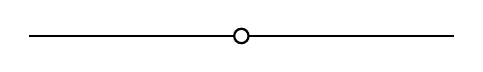
\begin{tikzpicture}[scale=1.0]
  \draw[thick] (-2.7,0) -- (2.7,0);
  \draw[thick,fill=white] (0,0) circle (2.6pt);
\end{tikzpicture}
\caption{原点加倍了的\trAffineLine{}。（依原书手绘图重绘。）}%
\label{fig:affine-line-doubled-origin}
\end{figure}

正如图画所暗示的，直观上这是\trHausdorff{}性质失效的一个类比。当然，$\mathbb{A}^1$ 本身并不是%
\trHausdorff{}的，所以我们不能说它是\trHausdorff{}性质的失效。我们觉得这事又古怪又糟糕，%
因此我们会想造出一个定义来防止这类事情发生。这将是\emph{\trSeparatedness}（separatedness）的观念%
（将在第~11~章中讨论）。（事实上，在某种意义上，\trSeparatedness{}才是\trHausdorff{}性质\emph{正确}的%
定义；见练习~11.2.B！）它还将应验我们在别处的祈祷。例如，在\trSeparated{}\trScheme{}上，%
「\trZariskiTopology{}的\trAffine\trBase」十分良好——两个\trAffine\trOpenSet{}的交将是\trAffine{}的%
（命题~11.2.13）。

\begin{exercise}\label{ex:doubled-origin-line-not-affine}
证明原点加倍了的\trAffineLine{}不是\trAffine{}的。提示：算出\trGlobalSections{}环，并回头看看关于%
$\mathbb{A}^2\smallsetminus\{(0,0)\}$ 的那个论证。
\end{exercise}

\begin{exercise}[容易的练习]\label{ex:doubled-origin-plane}
把同一构造中的 $\mathbb{A}^1$ 换成 $\mathbb{A}^2$ 再做一遍。你将定义出\textbf{原点加倍了的\trAffine{}平面}%
（affine plane with doubled origin）。描述这个\trScheme{}的两个\trAffine\trOpenSubset，使其交不是一个%
\trAffine\trOpenSubset。（这个例子已在警示~4.3.3 中被许诺。此外，「无穷维」版本将出现在练习~5.1.K 中。）
\end{exercise}

\textbf{4.4.6.\ 第三个例子：\trProjectiveLine{}。}\quad 考虑经由 $t\leftrightarrow 1/u$ 给出的\trIsomorphism{}%
$k[t,1/t]\overset{\sim}{\longrightarrow}k[u,1/u]$ 而来的 $U\cong V$。图~\ref{fig:gluing-p1}是这次粘合的%
一幅富有启发性的图。所得的\trScheme{}称为\textbf{\trField{} $k$ 上的\trProjectiveLine{}}%
（projective line over the field $k$），记作 $\mathbb{P}^1_k$。

\begin{figure}[htbp]
\centering
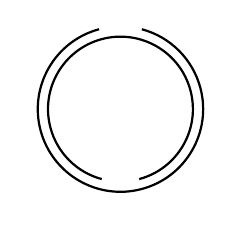
\begin{tikzpicture}[scale=1.0,line width=0.8pt]
  \draw (105:1.05) arc (105:435:1.05);
  \draw (285:0.92) arc (285:615:0.92);
\end{tikzpicture}
\caption{把两条\trAffineLine{}粘合起来得到 $\mathbb{P}^1$。（依原书手绘图重绘。）}%
\label{fig:gluing-p1}
\end{figure}

注意这些点是怎样粘合的。为方便起见，让我假设 $k$ 是\trAlgClosed{}的。（你可以想一想，若不然%
情况会如何改变。）在第一条\trAffineLine{}上，我们有闭的（「传统的」）点 $[(t-a)]$，我们把它想成%
「$t$-直线上的 $a$」，还有\trGenericPoint{} $[(0)]$。在第二条\trAffineLine{}上，我们有%
「$u$-直线上的 $b$」这样的\trClosedPoint，以及\trGenericPoint。于是，$t$-直线上的 $a$ 被粘到%
$u$-直线上的 $1/a$（当然，要求 $a\neq 0$），而\trGenericPoint{}被粘到\trGenericPoint（$k[t]$ 的%
\trIdeal{} $(0)$ 经\trLocalization{}后成为 $k[t,1/t]$ 的\trIdeal{} $(0)$，$k[u]$ 的\trIdeal{} $(0)$%
经\trLocalization{}后成为 $k[u,1/u]$ 的\trIdeal{} $(0)$；而在\trIsomorphism{} $t\longleftrightarrow 1/u$
之下，$k[t,1/t]$ 中的 $(0)$ 就是 $k[u,1/u]$ 中的 $(0)$）。

\textbf{4.4.7.}\quad 若 $k$ 是\trAlgClosed{}的，我们可以按下述方式解读 $\mathbb{P}^1_k$ 的%
\trClosedPoint{}——这也许会让你觉得，它更接近你先前见过的\trProjectiveSpace{}的定义方式。%
这些点形如 $[a,b]$，其中 $a$ 与 $b$ 不全为零，且 $[a,b]$ 被认同于 $[ac,bc]$，其中 $c\in k^{\times}$。%
那么，当 $b\neq 0$ 时，它被认同于 $t$-直线上的 $a/b$；当 $a\neq 0$ 时，它被认同于 $u$-直线上的 $b/a$。

\vkthmsync{8}
\begin{proposition}\label{thm:p1-not-affine}
$\mathbb{P}^1_k$ \emph{不是\trAffine{}的}。
\end{proposition}

\emph{证明。}\ 我们通过计算\trGlobalSections{}环来证明。\trGlobalSections{}对应于 $X$ 上的\trSection{}%
与 $Y$ 上的\trSection{}中在重叠处相互一致的那些。$X$ 上的一个\trSection{}是多项式 $f(t)$；%
$Y$ 上的一个\trSection{}是多项式 $g(u)$。把 $f(t)$ 限制到重叠上，得到的那个东西仍可称之为 $f(t)$；%
对 $g(u)$ 亦然。现在我们要求二者相等：$f(t)=g(1/t)$。但既是 $t$ 的多项式又是 $1/t$ 的多项式者，%
只有常值 $k$。于是 $\Gamma(\mathbb{P}^1,\OO_{\mathbb{P}^1})=k$。若 $\mathbb{P}^1$ 是\trAffine{}的，%
则它将是 $\Spec\Gamma(\mathbb{P}^1,\OO_{\mathbb{P}^1})=\Spec k$，也就是说，一个点。但它不是——%
它有许许多多的点。\hfill$\square$

我们由此证明了一条重要定理的类比：$\mathbb{CP}^1$ 上的\trHolomorphic{}函数只有常值函数！%
（关于一个严肃却又容易的推广，见 \S11.4.7。）

\textbf{4.4.9.\ 重要例子：\trProjectiveSpace。}\quad 我们现在给出\textbf{\trField{} $k$ 上的\trProjective{} $n$-空间}%
（projective $n$-space over a field $k$）的一个初步定义，记作 $\mathbb{P}^n_k$：把 $n+1$ 个%
\trOpenSet{}粘合起来，其中每一个都\trIsomorphic{}于 $\mathbb{A}^n_k$。为这些\trOpenSet{}择取明智的%
记号，会让我们的日子好过些。动机如下。在上述 $\mathbb{P}^1$ 的构造中，我们把\trProjectiveSpace{}的点%
想成 $[x_0,x_1]$，其中 $(x_0,x_1)$ 只在相差标量的意义下确定，即 $(x_0,x_1)$ 与%
$(\lambda x_0,\lambda x_1)$ 被视为相同。于是，第一张「卡」（patch）可以解读为：取 $x_0\neq 0$ 的%
那个\trLocus，然后考虑点 $[1,t]$，并把 $t$ 想成 $x_1/x_0$；尽管 $x_0$ 与 $x_1$ 都不是\trWellDefined{}的，%
$x_1/x_0$ 却是。第二张「卡」对应于 $x_1\neq 0$ 的情形：我们考虑点 $[u,1]$，并把 $u$ 想成 $x_0/x_1$。%
改用记号 $x_{1/0}$ 表示 $t$、$x_{0/1}$ 表示 $u$，将会很有用。

对 $\mathbb{P}^n$，我们把 $n+1$ 个\trOpenSet{}粘合起来，$i=0,\dots,n$ 各取其一。第 $i$ 个%
\trOpenSet{} $U_i$ 将具有坐标 $x_{0/i}$、……、$x_{(i-1)/i}$、$x_{(i+1)/i}$、……、$x_{n/i}$。%
采用写法
\begin{equation*}\tag{4.4.9.1}\label{eq:proj-patches-notation}
\Spec k[x_{0/i},x_{1/i},\dots,x_{n/i}]/(x_{i/i}-1)
\end{equation*}
会很方便。（这样我们引入了一个「哑变量」$x_{i/i}$，随即就把它取值为 $1$。）我们把 $U_i$ 的%
\trDistinguishedOpen{} $D(x_{j/i})$ 粘合到 $U_j$ 的\trDistinguishedOpen{} $D(x_{i/j})$ 上，办法是%
描述环的认同，从而认同这两个\trScheme：
\[
\begin{aligned}
&k[x_{0/i},x_{1/i},\dots,x_{n/i},1/x_{j/i}]/(x_{i/i}-1)\\
&\qquad\cong k[x_{0/j},x_{1/j},\dots,x_{n/j},1/x_{i/j}]/(x_{j/j}-1)
\end{aligned}
\]
认同方式为 $x_{k/i}=x_{k/j}/x_{i/j}$、$x_{k/j}=x_{k/i}/x_{j/i}$（这蕴涵 $x_{i/j}x_{j/i}=1$）。%
我们还需要检验：这份粘合信息在三重重叠处是相容的。

\begin{exercise}\label{ex:proj-triple-overlap}
尽可能不痛地检验这件事。（可能的提示：三重交是\trAffine{}的；请描述相应的环。）
\end{exercise}

\vkthmsync{10}
\begin{definition}[$\mathbb{P}^n_A$]\label{thm:projective-space-over-ring}
注意，我们的定义并未用到 $k$ 是\trField{}这一事实。因此，我们不妨对任意\emph{\trRing} $A$ 定义%
$\mathbb{P}^n_A$。这日后会派上用场。
\end{definition}

\begin{exercise}\label{ex:proj-functions-constant}
证明 $\mathbb{P}^n_k$ 上的函数只有常值函数（$\Gamma(\mathbb{P}^n_k,\OO)\cong k$），从而当 $n>0$ 时%
$\mathbb{P}^n_k$ 不是\trAffine{}的。提示：你也许会担心，需要在你的全部\trAffine\trOpenSet{}之间作某种精巧的%
相互配合；但其实，只需其中两个\trOpenSet{}便能看出这件事。这背后甚至还有几何直观：%
两个\trOpenSet{}之并的\trComplement{}\trCodimension{}为 $2$。而「\trAlgebraic{}\trHartogs{}引理」%
（在 \S4.4.2 中被非正式地讨论过，并将在定理~13.5.19 中得到严格陈述）说：定义在这个并上的任何函数%
都可延拓为整个\trProjectiveSpace{}上的函数。既然我们预期\trProjectiveSpace{}上的函数只有常值函数，%
那么在我们这两个\trAffine\trOpenSet{}的并上，这一点就应当已经显现了。
\end{exercise}

\begin{exercise}[推广 \S4.4.7]\label{ex:closed-points-pn-traditional}
证明：若 $k$ 是\trAlgClosed{}的，则 $\mathbb{P}^n_k$ 的\trClosedPoint{}可以按传统方式解读：%
点形如 $[a_0,\dots,a_n]$，其中诸 $a_i$ 不全为零，且 $[a_0,\dots,a_n]$ 被认同于%
$[\lambda a_0,\dots,\lambda a_n]$，其中 $\lambda\in k^{\times}$。
\end{exercise}

有益的翻译：我们把 $\mathbb{P}^n_k$（其中 $k=\overline{k}$）的\trClosedPoint{}想成%
$[x_0,x_1,\dots,x_n]$，其中 $x_i\in k$（诸 $x_i$ 不全为零），并对一切 $\lambda\in k^{\times}$ 把%
$[x_0,x_1,\dots,x_n]$ 认同于 $[\lambda x_0,\lambda x_1,\dots,\lambda x_n]$。于是，%
$[x_0,x_1,\dots,x_n]$ 对应于一条过原点的直线，而 $(x_{0/i},x_{1/i},\dots,x_{n/i})$ 就是这条直线与%
\trHyperplane{} $x_i=1$ 相交之处。

我们日后会给出\trProjectiveSpace{}的其他定义（定义~4.5.9、\S15.2.3），届时诸 $x_i$ 将被称为%
\emph{\trProjective{}坐标}（projective coordinates）。我们在这里给出的第一个定义，做起计算来常常很顺手；%
但它有些不自然之处——\trProjectiveSpace{}是高度对称的，而从我们目前的定义里看不出这一点。%
此外，正如H.~\trWeyl（[Wey, p.~90]）所指出的：「把数作为坐标引入，是一种暴力行为。」

\textbf{4.4.11.\ 有趣的题外话：\trChineseRemainderTheorem{}是一个\emph{几何}事实。}\quad \trChineseRemainderTheorem{}就嵌在我们%
做过的事情之中。我们将通过一个单独的例子看到这一点，但你随后应当把一般陈述自己想明白。%
\trChineseRemainderTheorem{}说：知道一个整数模 $60$ 的余数，与知道它模 $3$、$4$ 与 $5$ 的余数，是一回事。%
下面是用\trScheme{}的语言来看这件事的方式。$\Spec\mathbb{Z}/(60)$ 是什么？这个\trRing{}的\trPrimeIdeal{}%
有哪些？答：$\mathbb{Z}$ 中包含 $(60)$ 的那些\trPrimeIdeal，也就是整除 $60$ 的那些素数，%
即 $(2)$、$(3)$ 与 $(5)$。图~\ref{fig:spec-z-60}是 $\Spec\mathbb{Z}/(60)$ 的一幅草图。%
它们都是\trClosedPoint，因为这些都是\trMaximalIdeal，于是其\trTopology{}是\trDiscreteTopology。%
\trStalk{}是什么？你可以验证：它们是 $\mathbb{Z}/(4)$、$\mathbb{Z}/(3)$ 与 $\mathbb{Z}/(5)$。%
「在 $(2)$ 处」的\trNilpotent{}元由该点上的「\trFuzz{}」标示。（\S4.2 中我们讨论过用%
「无穷小\trFuzz{}」可视化\trNilpotent{}元。）那么这个\trScheme{}上的\trGlobalSections{}是什么？%
它们是「这个\trOpenSet{} $(2)$」「另一个\trOpenSet{} $(3)$」与「第三个\trOpenSet{} $(5)$」上的%
\trSection。换言之，我们有环的一个\trNaturalIsomorphism
\[
\mathbb{Z}/(60)\overset{\sim}{\longrightarrow}\mathbb{Z}/(2^2)\times\mathbb{Z}/(3)\times\mathbb{Z}/(5).
\]

\begin{figure}[htbp]
\centering
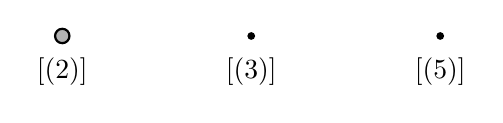
\begin{tikzpicture}[scale=1.0]
  \filldraw[fill=gray!60,line width=0.8pt] (0,0) circle (2.6pt);
  \fill (2.4,0) circle (1.4pt);
  \fill (4.8,0) circle (1.4pt);
  \node at (0,-0.45) {$[(2)]$};
  \node at (2.4,-0.45) {$[(3)]$};
  \node at (4.8,-0.45) {$[(5)]$};
\end{tikzpicture}
\caption{$\Spec\mathbb{Z}/(60)$ 的一幅图。（依原书手绘图重绘。）}%
\label{fig:spec-z-60}
\end{figure}

\vkthmsync{12}
\begin{example}[\extrahard]\label{thm:quadric-cone-section-example}
这是\trScheme{}的某个\trOpenSubset{}上一个函数的例子，其行为有些出人意料。在%
$X=\Spec k[w,x,y,z]/(wz-xy)$ 上考虑\trOpenSubset{} $D(y)\cup D(w)$。显然，$D(y)$ 上的函数 $z/y$ 与%
$D(w)$ 上的函数 $x/w$ 在重叠 $D(y)\cap D(w)$ 上一致。于是它们粘合起来给出一个\trSection。%
在\trComplexGeometry{}中思考\trAnalytic{}延拓（analytic continuation）时，你也许见过这种局面——我们有一个%
「\trHolomorphic{}」函数，它在某个\trOpenSet{}上由 $z/y$ 描述，而这个描述在别处失效，但你仍可以通过让这个%
函数在空间的不同部分取不同的定义，来对它进行「\trAnalytic{}延拓」。
\end{example}

\emph{给好奇行家的后续讨论。}\ 这个函数没有任何用 $w$、$x$、$y$、$z$ 表出的「单一描述」可以成为%
\trWellDefined{}的表达式！这里有大量有趣的几何，而这个\trScheme{}将是我们取之不竭的（反）例来源%
（在索引中查「反复登场的（反）例」）。下面用它尚未定义的语言，先给你惊鸿一瞥。空间%
$\Spec k[w,x,y,z]$ 是 $\mathbb{A}^4$，不出所料，是四维的。我们打交道的对象是子集 $X$，它是一张%
\trHypersurface，是三维的。它是 $\mathbb{P}^3$ 中一张\trSmooth\trQuadricSurface{}上的\trCone%
（翻到图~9.2）。\trOpenSubset{} $D(y)\subset X$ 是 $X$ 减去某张\trHypersurface，所以我们扔掉的%
是一个\trCodimension{} $1$ 的\trLocus。\trOpenSubset{} $D(w)$ 则还要扔掉另一个\trCodimension{} $1$ 的\trLocus。%
你也许会想：这两块被丢弃的\trLocus{}之交于是\trCodimension{}为 $2$，而这个古怪函数之所以不能延拓为%
整体多项式，是因为我们那条\trHartogs{}引理型的定理失效了。但事实并非如此——%
$V(y)\cap V(w)$ 其实\trCodimension{}为 $1$。实际发生的情况如下。空间 $V(y)$ 的得到方式，是扔掉%
（两条直线 $\ell$ 与 $m_1$ 之并上的）\trCone，这两条直线在\trSurface{}的两族「\trRuling{}」（ruling）中各居其一；\footnote{译注：此处原文作 $V(y)$；按数学内容，如此「扔掉锥」所得的空间应为 $D(y)$。}%
$V(w)$ 同样涉及扔掉（两条直线 $\ell$ 与 $m_2$ 之并上的）\trCone。其交是（直线 $\ell$ 上的）\trCone，%
这是一个\trCodimension{} $1$ 的\trSet。令人称奇的是：尽管它是「纯\trCodimension{} $1$」的，$\ell$ 上的这个\trCone{}却%
连作为\trSet{}都无法由单个方程割出（见练习~15.5.N）。这意味着：对我们的函数而言，任何形如%
$f(w,x,y,z)/g(w,x,y,z)$ 的表达式都不能正确描述它在 $D(y)\cup D(w)$ 上的取值——在%
$D(y)\cup D(w)$ 的某一点处，它必定是 $0/0$。缘由如下。我们的函数无法定义在 $V(y)\cap V(w)$ 上，%
所以 $g$ 必须在这里消失。但 $g$ 不能只在 $\ell$ 上的\trCone{}处消失——它必须在别处也消失。


\section{\trProjectiveScheme{}与$\Proj$构造}

\trProjectiveScheme{}之重要，有几个理由，这里举出几条。几何中那些具有「经典趣味」的\trScheme——以及你在还不知\trScheme{}为何物时就该会关心的那些\trScheme——全是\trProjective{}的，或是\trProjective{}者的\trOpenSubset（基本上就是\emph{\trQuasiprojective}（quasiprojective）的；见 \S4.5.10）。此外，大多数「令人感兴趣的\trScheme」也趋于\trProjective{}或\trQuasiprojective。事实上，哪怕是举出一个例子：一个满足基本性质——比如说，在\trField{}上\trFiniteType{}且「\trHausdorff」（即「\trSeparated」）——却可证明不是\trQuasiprojective{}的\trScheme，都是极难的。对做复几何的人：很难找到一个可证明非\trProjective{}的\trCompact\trComplex\trVariety（见\mbox{注记~11.4.6}），也很难造出一个可证明不是「\trProjective\trVariety{}的\trOpenSubset」的复\trVariety。所以\trProjectiveScheme{}实在无处不在。再者，「\trProjective{} $k$-\trScheme」这一概念，是\trCompactness{}之代数几何版本（即「\trProperness{}」（properness）；见 \S11.4）的一个良好近似。

最后，尽管\trProjectiveScheme{}可以由\trAffineScheme{}粘合而成，而且我们也知道追踪粘合是件烦人的事，但有一种不必操心粘合的简单办法来对付它们。正如\trRing{}与\trAffineScheme{}之间存在一部粗糙的词典，\trGradedRing{}与\trProjectiveScheme{}之间也将有一部（稍宽松些的）类比词典。正如人们能以\trRing{}代\trAffineScheme{}而工作，人们也能以\trGradedRing{}代\trProjectiveScheme{}而工作。

\textbf{4.5.1.\ 来自经典几何的动机。}\quad 为得几何直观，我们回忆一下人们如何「经典地」思考\trProjectiveSpace（在实数上、带\trClassicalTopology）。$\mathbb{P}^n$ 可以被解读为 $\mathbb{R}^{n+1}$ 中过原点的诸直线。于是 $\mathbb{P}^n$ 的子集对应于 $\mathbb{R}^{n+1}$ 中过原点的一些直线之并，而\trClosedSubset{}对应的则是其中为\trClosedSet{}的那些并。（若把「闭」换成「开」，同样的说法便不成立！）

人们常把 $\mathbb{P}^n$ 想象成 $\mathbb{R}^{n+1}$ 中「无穷远处」的那些点：沿一个方向无穷远的点，与沿相反方向无穷远的点被联系在一起。利用分解式
\[
\mathbb{P}^{n+1}=\mathbb{R}^{n+1}\amalg\mathbb{P}^n,
\]
可以把这件事说得更精确：它的意思是，$\mathbb{P}^{n+1}$ 中有一个\trOpenSubset{}被认同于 $\mathbb{R}^{n+1}$（最后一个「\trProjective\trCoordinate」非零的那些点），而余下的\trClosedSubset{}则被认同于 $\mathbb{P}^n$（最后一个「\trProjective\trCoordinate」为零的那些点）。（「\trProjective\trCoordinate」一语要到 \S4.5.9 才正式定义，但我们在那之前就会用它，见\cref{ex:conic-via-standard-charts}与\cref{ex:cut-out-by-forms}。）

举例来说，在 $\mathbb{P}^n$ 中切出某个点集 $V$ 的任何方程，也会在 $\mathbb{R}^{n+1}$ 中切出某个点集，它将是过原点的诸直线之闭并。我们称之为 $V$ 的\emph{\trAffine\trCone}（affine cone）。这些方程还会在 $\mathbb{P}^{n+1}$ 中切出由一簇 $\mathbb{P}^1$ 组成的并，我们称之为 $V$ 的\emph{\trProjective\trCone}（projective cone）。\trProjective\trCone{}正是\trAffine\trCone{}与 $V$ 的\trDisjointUnion。例如，$\mathbb{P}^2$ 中 $x^2+y^2=z^2$ 的\trAffine\trCone，正是 $\mathbb{R}^3$ 中锥面的那幅「经典」图像；见图~\ref{fig:affine-projective-cone}。我们将在 \S9.3.11 于代数的场景中把这一类比做精确。

\begin{figure}[htbp]
\centering
\begin{tikzpicture}[scale=0.92,every node/.style={font=\small}]
  \draw[thick] (0,0) circle (1.5);
  \draw[dotted,thick] (0,-0.1) ellipse (1.46 and 0.3);
  \draw[thick] (-0.73,0.92) -- (0,0.02) -- (0.73,0.92);
  \draw[thick] (0,0.92) ellipse (0.73 and 0.17);
  \draw[thick] (-0.73,-0.92) -- (0,0.02) -- (0.73,-0.92);
  \draw[thick] (0,-0.92) ellipse (0.73 and 0.17);
  \node[anchor=west] at (1.75,1.7) {$x^2+y^2=z^2$（在 $\mathbb{P}^2$ 中）};
  \draw[dashed,->] (1.7,1.6) -- (0.18,1.02);
  \draw[dashed,->] (1.7,1.56) -- (-0.4,1.0);
  \node[anchor=west] at (1.9,0.85) {$\mathbb{P}^3$ 中的\trProjective\trCone};
  \draw[dashed,->] (1.85,0.85) -- (0.7,0.97);
  \node[anchor=west] at (2.15,-0.2) {\trAffine\trCone：$x^2+y^2=z^2$（在 $\mathbb{R}^3$ 中）};
  \draw[dashed,->] (2.1,-0.16) -- (0.42,0.54);
\end{tikzpicture}
\caption{经典几何中 $x^2+y^2=z^2$ 的\trAffine\trCone{}与\trProjective\trCone。（依原书手绘图重绘。）}\label{fig:affine-projective-cone}
\end{figure}

\textbf{4.5.2.\ \trProjectiveScheme：第一份描述。}\quad 我们现在来描述\trProjectiveScheme{}的一种构造，它将有助于为$\Proj$构造提供动机。我们先把刚才描述的锥作代数解读，更一般地，也来练习一番「在诸\trProjective\trCoordinate{}之间」与「在标准\trAffine\trOpenSubset{}上的坐标」之间的换算。我们把坐标从 $x$、$y$、$z$ 换成 $x_0$、$x_1$、$x_2$，以便使用 \S4.4.9 的记号。对下面的诸问题，在 $\mathbb{P}^2_k$ 中取\trProjective\trCoordinate{} $x_0$、$x_1$、$x_2$。（「\trProjective\trCoordinate」这个术语到 \S4.5.9 才正式定义，但这些练习你反正应当能做。）大\trOpenSet（或曰「坐标卡」（coordinate chart））$U_0=\{[x_0,x_1,x_2]\ :\ x_0\neq0\}$ 带有坐标 $x_{1/0}$ 与 $x_{2/0}$，我们把它们解读为 $x_1/x_0$ 与 $x_2/x_0$。$U_1$ 与 $U_2$ 也有类似的定义。为方便起见，约定 $x_{0/0}$ 为 $1$。

\begin{exercise}\label{ex:proj-coordinate-change}
用 $(x_{1/0},x_{2/0})$ 描述 $(x_{0/1},x_{2/1})$。
\end{exercise}

\begin{exercise}\label{ex:conic-via-standard-charts}
解释如何定义一个\trScheme，它应被解读为「『在 $\mathbb{P}^2_k$ 中』的 $x_0^2+x_1^2-x_2^2=0$」。提示：在 $x_2\neq0$ 所对应的\trAffine\trOpenSubset{}中，它应当（用 \S4.4.9 的语言）由 $x_{0/2}^2+x_{1/2}^2-1=0$ 切出，也就是说，它应当「就是」\trScheme{} $\Spec k[x_{0/2},x_{1/2}]/(x_{0/2}^2+x_{1/2}^2-1)$。你可以同样猜出它在另外两个标准\trOpenSet{}上应当是什么，并证明这三个\trScheme{}能够粘合在一起。
\end{exercise}

\begin{exercise}\label{ex:dehomogenization}
(a)~描述 $x_0$、$x_1$、$x_2$ 的\emph{所有}那些能被「去齐次化」（dehomogenized）为 $x_{1/0}^2+x_{2/0}^5=1$ 的\trHomogeneous{}多项式，并解释其中哪一个是「最好的」。

(b)~这些多项式的\trVanishingSet{}与 $\mathbb{P}^2_k$ 中的「\trLineAtInfinity」（line at infinity）$x_0=0$ 相交于哪些点？
\end{exercise}

\begin{exercise}\label{ex:parabola-at-infinity}
考虑抛物线 $x_{2/0}=x_{1/0}^2$（或者随你所好，$y=x^2$）。它与\trLineAtInfinity{}如何相交？（这是什么意思？）它在各个\trCoordinatePatch{} $U_1$ 与 $U_2$ 中的描述又是什么？
\end{exercise}

\textbf{4.5.3.}\ \emph{\trhRemark{}：$\mathbb{P}^n$ 中的次数 $d$ \trHypersurface。}\quad \trField{}上 $n+1$ 个变量的次数 $d$ \trHomogeneous{}多项式构成一个 $\binom{n+d}{d}$ 维\trVectorSpace。（这基本上就是\mbox{练习~9.3.J}与\mbox{练习~15.1.C}的内容。）「两个多项式切出 $\mathbb{P}^n_k$ 的同一个子集，当且仅当其中一个是另一个的非零标量倍」——这话几乎是真的。遗憾的是，$x^2y=0$ 与 $xy^2=0$ 这两个例子表明「仅当」并不总成立。日后你将能够验证（例如用\mbox{练习~9.5.C}）：两个多项式切出同一个\emph{\trClosedSubscheme}（不论那是什么意思），当且仅当其中一个是另一个的非零标量倍。（这是「\trClosedSubscheme」这一观念优于「\trClosedSubset」的某种证据。）零多项式无论按这个词的哪种合理解读，都谈不上真正切出一张\trHypersurface。于是我们不严格地想象：「$\mathbb{P}^n$ 中次数 $d$ 的\trHypersurface{}由 $\mathbb{P}^{\binom{n+d}{d}-1}$ 参数化」。这一直觉将（在特殊情形中）反复出现，我们将在 \S25.3.5 赋予它精确的含义。（要等有了\trClosedSubscheme{}的语言，我们才会在 \S9.3.2 正式定义\trHypersurface；届时我们还会定义直线、\trHyperplane{}（hyperplane）、二次超曲面、\trConic{}（conic curve），以及其他种种奇妙的观念。）

\begin{exercise}[推广\cref{ex:conic-via-standard-charts}的练习]\label{ex:cut-out-by-forms}
考虑带\trProjective\trCoordinate{} $x_0,\dots,x_n$ 的 $\mathbb{P}^n_A$。给定一组\trHomogeneous{}多项式 $f_i\in A[x_0,\dots,x_n]$，请为「在 $\mathbb{P}^n_A$ 中由诸 $f_i$ 切出的\trScheme」这一说法赋予意义。（日后将把这件事精确化为\trVanishingScheme（vanishing scheme）的一个例子；见\cref{ex:vanishing-scheme-definition}。）
\end{exercise}

这一句本来就可以当作\emph{\trProjective{} $A$-\trScheme}的定义，但我们要按兵不动，留到 \S4.5.10 再把它陈述得稍好一些。

\textbf{4.5.4.\ 关于\trGradedRing{}的预备知识。}\quad $\Proj$构造从一个\trGradedRing{}造出一个\trScheme。我们现在给出一些关于\trGradedRing{}的背景知识。

\textbf{4.5.5.}\ \emph{定义：$\mathbb{Z}$-\trGradedRing。}\quad 一个\textbf{$\mathbb{Z}$-\trGradedRing}（$\mathbb{Z}$-graded ring）是一个\trRing{} $S_\bullet=\oplus_{n\in\mathbb{Z}}S_n$（该下标称为\textbf{\trGrading}（grading）），其乘法与\trGrading{}相容，即把 $S_m\times S_n$ 送入 $S_{m+n}$。显然 $S_0$ 是一个\trSubring，每个 $S_n$ 都是 $S_0$-\trModule，而 $S_\bullet$ 是一个 $S_0$-\trAlgebra。在本 \S4.5.5 的其余部分，设 $S_\bullet$ 是一个 $\mathbb{Z}$-\trGradedRing。诸个别 $S_n$ 中的元素称为 $S_\bullet$ 的\textbf{\trHomogeneous{}元素}（homogeneous elements）。$S_\bullet$ 的一个\trIdeal{} $I$ 称为\textbf{\trHomogeneous\trIdeal}（homogeneous ideal）（或称\trGradedIdeal{}（graded ideal），不过我们不会使用这个术语），如果它由\trHomogeneous{}元素生成。非零的\trHomogeneous{}元素带有显然的\textbf{次数}（degree）。$S_d$ 中的元素称为\textbf{次数 $d$ 的\trForm}（form of degree $d$）。

\begin{exercise}\label{ex:homogeneous-ideal-basics}
(a)~证明：一个\trIdeal{} $I$ 是\trHomogeneous\trIdeal，当且仅当对每个 $n$，它都含有其每个元素的次数 $n$ 分片。（于是 $I$ 可以分解为\trHomogeneous{}分片 $I=\oplus I_n$，且 $S_\bullet/I$ 带有自然的 $\mathbb{Z}$-\trGrading。这正是「\trHomogeneous\trIdeal」之名的缘由。）

(b)~证明：给定的 $\mathbb{Z}$-\trGradedRing{} $S_\bullet$ 的全体\trHomogeneous\trIdeal{}这一集合，对和、积、交与\trRadical{}封闭。

(c)~设 $I\subset S_\bullet$ 是\trHomogeneous\trIdeal。证明：若 $I\neq S_\bullet$，并且对任意\trHomogeneous{}的 $a$, $b\in S_\bullet$，只要 $ab\in I$ 就有 $a\in I$ 或 $b\in I$，则 $I$ 是\trPrimeIdeal。

若 $T$ 是 $S_\bullet$ 的一个只含\trHomogeneous{}元素的\trMultiplicativeSubset，则 $T^{-1}S_\bullet$ 自然带有 $\mathbb{Z}$-\trGradedRing{}结构。
\end{exercise}

\textbf{4.5.6.}\ \emph{$\mathbb{Z}^{\ge0}$-\trGradedRing、$A$ 上的\trGradedRing{}与\trFinitelyGenerated{}的\trGradedRing。}\quad 一个 $\mathbb{Z}^{\ge0}$-\trGradedRing{}是不含负次数元素的 $\mathbb{Z}$-\trGradedRing。

\textbf{在本书的其余部分，\trGradedRing{}一词均指 $\mathbb{Z}^{\ge0}$-\trGradedRing。警告：这一约定是非标准的（而且自有其理由）。}

从今往后，除非另有声明，$S_\bullet$ 均被默认为\trGradedRing。取定一个\trRing{} $A$，我们称之为\textbf{\trBaseRing}（base ring）。若 $S_0=A$，我们就说 $S_\bullet$ 是 $A$ 上的\textbf{\trGradedRing}（graded ring over $A$）。一个关键例子是 $A[x_0,\dots,x_n]$，或者更一般地 $A[x_0,\dots,x_n]/I$，其中 $I$ 是满足 $I\cap S_0=0$ 的\trHomogeneous\trIdeal（参\cref{ex:cut-out-by-forms}）。这里对 $A[x_0,\dots,x_n]$ 取通常的\trGrading，即每个 $x_i$ 的权都是 $1$。

子集 $S_+:=\oplus_{i>0}S_i\subset S_\bullet$ 是一个\trIdeal，称为\textbf{\trIrrelevantIdeal}（irrelevant ideal）。「无关」之名的缘由，再过几段自会清楚。若\trIrrelevantIdeal{} $S_+$ 是一个\trFinitelyGenerated{}的\trIdeal，我们就说 $S_\bullet$ 是 $A$ 上的\textbf{\trFinitelyGenerated\trGradedRing}（finitely generated graded ring over $A$）。若 $S_\bullet$ 作为 $A$-\trAlgebra{}由 $S_1$ 生成，我们就说 $S_\bullet$ 是\textbf{在次数 $1$ 处生成的}（generated in degree 1）。（日后我们会发现，把「$S_\bullet$ 在次数 $1$ 处生成」解读为「自然映射 $\mathrm{Sym}^{\bullet}S_1\to S_\bullet$ 是\trSurjectiveMap」会很有用。\emph{\trSymmetricAlgebra}（symmetric algebra）这一构造将在 \S14.2.6 中简略讨论。）

\begin{exercise}\label{ex:fg-graded-rings}
(a)~证明：$A$ 上的\trGradedRing{} $S_\bullet$ 是（$A$ 上的）\trFinitelyGenerated\trGradedRing，当且仅当 $S_\bullet$ 是\trFinitelyGenerated{}的\trGrading{} $A$-\trAlgebra，也就是说，它由 $A=S_0$ 添上有限多个正次数的\trHomogeneous{}元素生成。（正向蕴涵的提示：证明 $S_+$ 作为\trIdeal{}的\trGenerator，同时也是 $S_\bullet$ 作为\trAlgebra{}的\trGenerator。）

(b)~证明：$A$ 上的\trGradedRing{} $S_\bullet$ 是\trNoetherian{}的，当且仅当 $A=S_0$ 是\trNoetherian{}的，且 $S_\bullet$ 是\trFinitelyGenerated{}的\trGradedRing。
\end{exercise}

\textbf{4.5.7.\ $\Proj$构造。}\quad 我们现在来定义一个\trScheme{} $\Proj S_\bullet$，其中 $S_\bullet$ 是（$\mathbb{Z}^{\ge0}$-）\trGradedRing。这里先给出两个例子，好让隧道尽头先透出一点亮光。若 $S_\bullet=A[x_0,\dots,x_n]$，我们将会复原出 $\mathbb{P}^n_A$；而若 $S_\bullet=A[x_0,\dots,x_n]/(f(x_0,\dots,x_n))$，其中 $f$ 是\trHomogeneous{}的，我们将会构造出某个「在 $\mathbb{P}^n_A$ 中由方程 $f=0$ 切出」的东西（参\cref{ex:cut-out-by-forms}）。

正如我们对\trRing{}的 $\Spec$ 所做的那样，我们将先把 $\Proj S_\bullet$ 造为集合，再造为\trTopologicalSpace，最后造为\trRingedSpace。在对 $\mathbb{P}^n_A$ 的初步定义中，我们把 $n+1$ 片精心挑选的\trAffine{}拼片粘合在一起；但我们不想做任何选取，于是改为同时考虑「一切可能」的\trAffine\trOpenSet{}来做这件事。我们的\trAffine{}砌块将如下。对每个\trHomogeneous{}的 $f\in S_+$，注意\trLocalization{} $(S_\bullet)_f$ 自然是一个 $\mathbb{Z}$-\trGradedRing，其中 $\deg(1/f)=-\deg f$。考虑
\begin{equation*}\tag{4.5.7.1}\label{eq:spec-localized-zero-graded}
\Spec((S_\bullet)_f)_0,
\end{equation*}
其中 $((S_\bullet)_f)_0$ 表示\trGradedRing{} $(S_\bullet)_f$ 的次数 $0$ 分片。（当 $f$ 跑遍 $S_+$ 的全部\trHomogeneous{}元素时，这些 $((S_\bullet)_f)_0$ 将是我们的\trAffine{}砌块。）记号 $((S_\bullet)_f)_0$ 坦白说糟糕透顶——第一个与第三个下标关乎\trGrading，第二个则关乎\trLocalization。至于为何要考虑这一构造，这里给出动机：把它应用到 $S_\bullet=k[x_0,\dots,x_n]$、$f=x_i$，便得到出现于 \eqref{eq:proj-patches-notation} 中的那个\trRing
\[
k[x_{0/i},x_{1/i},\dots,x_{n/i}]/(x_{i/i}-1).
\]

（在开始构造之前：定义 $\Proj S_\bullet$ 的另一条可能路径，是把这种形状的\trAffineScheme{}直接粘合起来——你可以径直跳到\cref{ex:pairwise-gluing-affines}与\cref{ex:triple-overlap-proj}。你若偏爱那条路，尽管自便。）

$\Proj S_\bullet$ 的\emph{点}，是 $S_\bullet$ 的那些不包含\trIrrelevantIdeal{} $S_+$ 的\trHomogeneous\trPrimeIdeal（即「相关的\trHomogeneous\trPrimeIdeal」（relevant homogeneous prime ideals））。

\begin{exercise}[重要而棘手的练习]\label{ex:zero-piece-prime-bijection}
设 $f\in S_+$ 是\trHomogeneous{}的。

(a)~给出 $((S_\bullet)_f)_0$ 的诸\trPrimeIdeal{}与 $(S_\bullet)_f$ 的诸\trHomogeneous\trPrimeIdeal{}之间的一个\trBijection。提示：为避免记号上的混淆，改为证明：若 $A_\bullet$ 是一个 $\mathbb{Z}$-\trGradedRing，带有一个\trInvertible{}的正次数\trHomogeneous{}元素 $f$，那么 $A_0$ 的诸\trPrimeIdeal{}与 $A_\bullet$ 的诸\trHomogeneous\trPrimeIdeal{}之间存在\trBijection。利用\trRingMorphism{} $A_0\to A_\bullet$，从 $A_\bullet$ 的每个\trHomogeneous\trPrimeIdeal{} $P$ 得到 $A_0$ 的一个\trPrimeIdeal{} $P_0:=P\cap A_0$。反方向：对 $A_0$ 的每个\trPrimeIdeal{} $P_0$，证明 $P:=\sqrt{P_0A_\bullet}$ 是 $A_\bullet$ 的\trPrimeIdeal。务必证明这两个映射的确构成\trBijection！

(b)~把 $((S_\bullet)_f)_0$ 的\trPrimeIdeal{}之集解读为 $\Proj S_\bullet$ 的一个子集。
\end{exercise}

$\Proj S_\bullet$ 的点与\trHomogeneous\trPrimeIdeal{}之间的这一对应，有助于我们对 $\Proj S_\bullet$ 形成图景。例如，设 $S_\bullet=k[x,y,z]$ 带通常的\trGrading，我们先把这个\trHomogeneous\trPrimeIdeal{} $(z^2-x^2-y^2)$ 想象成 $\Spec S_\bullet$ 的一个子集；它是一个\trCone（见图~\ref{fig:affine-projective-cone}）。如 \S4.5.1 中那样，我们把 $\mathbb{P}^2_k$ 想象成「\trPlaneAtInfinity」（plane at infinity）。于是我们把这条方程想象成在「无穷远处」切出一条\trConic（于 $\Proj S_\bullet$ 中）。我们将在 \S9.3.11 把这一直觉说得稍微精确些。

\textbf{4.5.8.}\quad 仿照仿射情形，若 $T$ 是 $S_\bullet$ 的一组\trHomogeneous{}元素，定义 $T$ 的（射影）\textbf{\trVanishingSet}：$V(T)\subset\Proj S_\bullet$，即那些包含 $T$ 但不包含 $S_+$ 的\trHomogeneous\trPrimeIdeal。若 $I$ 是\trHomogeneous\trIdeal，则以同样的方式定义 $V(I)$；注意它就等于 $V(T)$，其中 $T$ 是 $I$ 的任意一组\trHomogeneous\trGenerator。

若 $f$ 是正次数的\trHomogeneous{}元素，则按显而易见的方式定义 $V(f)$。令 $D_+(f):=\Proj S_\bullet\smallsetminus V(f)$（\textbf{\trProjective\trDistinguishedOpen}（projective distinguished open set）），即 $V(f)$ 的\trComplement。（这个下标意在把该记号与相仿的 $D(f)$ 区别开。）一旦我们在 $\Proj S_\bullet$ 上定义了\trScheme{}结构，我们就会（不加声明地）用 $D_+(f)$ 指称那个\trOpenSubscheme，而不只是\trOpenSubset。（虽然 $D_+(f)$ 的定义即便在 $f$ 次数为 $0$ 时也有意义，但我们有意只允许正次数的 $f$。例如，我们会希望诸 $D_+(f)$ 构成一张\trAffine\trCover；而若 $f$ 的次数为 $0$，$D_+(f)$ 就未必是\trAffine{}的了。）

\begin{exercise}\label{ex:d-plus-is-spec}
证明 $D_+(f)$「就是」（或者更精确地说，「对应于」）你在\cref{ex:zero-piece-prime-bijection}(b) 中描述的那个子集 $\Spec((S_\bullet)_f)_0$。例如在 \S4.4.9 中，诸 $D_+(x_i)$ 正是覆盖\trProjectiveSpace{}的标准\trOpenSet。
\end{exercise}

与仿射情形一样，诸 $V(I)$ 满足某一\trTopology{}的诸\trClosedSet{}之公理，我们称之为 $\Proj S_\bullet$ 上的\textbf{\trZariskiTopology}。（文献中给出的其他定义看上去也许貌异，但不难证明它们相同。）关于\trRing{}之 $\Spec$ 上\trZariskiTopology{}的许多论断，只需极少额外工夫便可搬到眼下这种情况。显然 $D_+(f)\cap D_+(g)=D_+(fg)$，其论证与仿射情形如出一辙（\cref{ex:distinguished-opens-intersection}）。

\begin{exercise}[容易的练习]\label{ex:d-plus-base}
验证诸\trProjective\trDistinguishedOpen{} $D_+(f)$（$f$ 跑遍 $S_+$ 的全部\trHomogeneous{}元素）构成\trZariskiTopology{}的一组\trBase。
\end{exercise}

\begin{exercise}\label{ex:proj-vanishing-ideals}
取定一个\trGradedRing{} $S_\bullet$。

(a)~设 $I$ 是 $S_\bullet$ 的含于 $S_+$ 的任一\trHomogeneous\trIdeal，$f$ 是一个正次数的\trHomogeneous{}元素。证明：$f$ 在 $V(I)$ 上消失（即 $V(I)\subset V(f)$），当且仅当对某个 $n$ 有 $f^n\in I$。（提示：模仿仿射情形；见\cref{ex:vanish-on-vi-radical}。）特别地，正如仿射情形（\cref{ex:distinguished-open-inclusion}）那样：若 $D_+(f)\subset D_+(g)$，则对某个 $n$ 有 $f^n\in(g)$，反之亦然。（这里 $g$ 也是正次数的\trHomogeneous{}元素。）

(b)~若 $Z\subset\Proj S_\bullet$，定义 $I(Z)\subset S_\bullet$。证明它是 $S_\bullet$ 的一个\trHomogeneous\trIdeal。对任意两个子集，证明 $I(Z_1\cup Z_2)=I(Z_1)\cap I(Z_2)$。

(c)~对任意子集 $Z\subset\Proj S_\bullet$，证明 $V(I(Z))=\overline{Z}$。
\end{exercise}

\begin{exercise}[参看\cref{ex:distinguished-cover-unit-ideal}]\label{ex:empty-vanishing-equivalents}
取定一个\trGradedRing{} $S_\bullet$ 与一个\trHomogeneous\trIdeal{} $I\subseteq S_+$。证明下列三条等价：
\begin{itemize}[label={},leftmargin=2.2em,itemsep=2pt,topsep=3pt]
\item (a)~$V(I)=\varnothing$。
\item (b)~对任何生成 $I$ 的\trHomogeneous{}元 $f_i$（$i$ 跑遍某个\trIndexSet），都有 $\cup D_+(f_i)=\Proj S_\bullet$。
\item (c)~$\sqrt{I}\supset S_+$。
\end{itemize}
这再次为 $S_+$ 之「无关」提供了动机：任何\trRadical{}包含它的\trIdeal{}都是「几何上无关的」。
\end{exercise}

我们现在把 $\Proj S_\bullet$ 造为\emph{\trScheme}。

\begin{exercise}\label{ex:zariski-restriction-d-plus}
设给定某个\trHomogeneous{}的 $f\in S_+$。经由\cref{ex:d-plus-is-spec}中的\trInclusionMap
\[
D_+(f)=\Spec((S_\bullet)_f)_0\lhook\joinrel\longrightarrow\Proj S_\bullet
\]
证明：$\Proj S_\bullet$ 上的\trZariskiTopology{}限制到 $\Spec((S_\bullet)_f)_0$ 上，正是 $\Spec((S_\bullet)_f)_0$ 自身的\trZariskiTopology。
\end{exercise}

至此我们已把 $\Proj S_\bullet$ 定义为\trTopologicalSpace，可以着手定义\trStructureSheaf{}了。在 $D_+(f)$ 上，我们希望它就是 $\Spec((S_\bullet)_f)_0$ 的\trStructureSheaf。我们将用\cref{ex:gluing-sheaves-cocycle}（关于粘合层的那条练习）把这些\trSheaf{}粘合起来。

\begin{exercise}\label{ex:pairwise-gluing-affines}
若 $f$, $g\in S_+$ 是\trHomogeneous{}且非零的，描述 $\Spec((S_\bullet)_{fg})_0$ 与 $\Spec((S_\bullet)_f)_0$ 的\trDistinguishedOpen{}子集 $D(g^{\deg f}/f^{\deg g})$ 之间的一个\trIsomorphism。
\end{exercise}

类似地，$\Spec((S_\bullet)_{fg})_0$ 也被认同于 $\Spec((S_\bullet)_g)_0$ 的一个\trDistinguishedOpen{}子集。于是我们便用这些两两粘合，把诸 $\Spec((S_\bullet)_f)_0$（$f$ 变动）粘合在一起。

\begin{exercise}\label{ex:triple-overlap-proj}
通过核查这些粘合在三重叠上表现良好（见\cref{ex:gluing-sheaves-cocycle}），完成\trScheme{} $\Proj S_\bullet$ 的定义。
\end{exercise}

\begin{exercise}\label{ex:proj-sheaf-compatible-germs}
（有人会觉得这条必不可少，也有人宁可视而不见。）用\trCompatibleGerm{}（重新）解读 $\Proj S_\bullet$ 的\trStructureSheaf。
\end{exercise}

\textbf{4.5.9.}\ \emph{\trhDefinition{}。}\quad 我们（重新）定义\textbf{\trProjectiveSpace}（\trRing{} $A$ 上的）为
\[
\mathbb{P}^n_A:=\Proj A[x_0,\dots,x_n].
\]
这一定义既不牵涉烦琐的粘合，也不牵涉对拼片的特殊选取。注意：诸变量 $x_0,\dots,x_n$——我们称之为 $\mathbb{P}^n_A$ 上的\textbf{\trProjective\trCoordinate}（projective coordinates）——是定义的一部分。（视上下文而定，它们也可以不叫 $x_i$ 而叫别的名字。）

\begin{exercise}\label{ex:proj-agrees-preliminary}
核查这与我们先前对 $\mathbb{P}^n_A$ 的构造（\S4.4.9）相一致。（你怎么知道诸 $D_+(x_i)$ 覆盖 $\Proj A[x_0,\dots,x_n]$？）
\end{exercise}

不难注意到：若按旧的\trProjectiveSpace{}定义，要证明 $D_+(x^2+y^2-z^2)\subset\mathbb{P}^2_k$（一条平面\trConic{}的\trComplement）是\trAffine{}的，会是一道并不平凡的练习；而有了新的视角，此事立等可取——它就是 $\Spec(k[x,y,z]_{(x^2+y^2-z^2)})_0$。

\begin{exercise}\label{ex:classical-point-homogeneous-prime}
设 $k$ 是\trAlgClosedField。由\cref{ex:closed-points-pn-traditional}我们知道，按 \S4.4.9 定义的 $\mathbb{P}^n_k$，其\trClosedPoint{}与「经典」\trProjectiveSpace{}的点成\trBijection。由\cref{ex:proj-agrees-preliminary}，按 \S4.4.9 定义的\trScheme{} $\mathbb{P}^n_k$\trIsomorphic{}于 $\Proj k[x_0,\dots,x_n]$。于是，经典\trProjectiveSpace{}的每个点 $[a_0,\dots,a_n]$ 都对应于 $k[x_0,\dots,x_n]$ 的一个\trHomogeneous\trPrimeIdeal。它是哪一个\trHomogeneous\trPrimeIdeal？
\end{exercise}

现在我们来弄清\trVanishingScheme{}的「正确定义」，以类比\trVanishingSet{} $V(\cdot)$（\S3.4.1）。你将在其中定义一个\trClosedSubscheme（注记~4.3.5 中已提及，其正式定义见 \S9.1）。

\begin{exercise}\label{ex:vanishing-scheme-definition}
若 $S_\bullet$ 在次数 $1$ 处生成，且 $f\in S_+$ 是\trHomogeneous{}的，解释如何在 $\Proj S_\bullet$「之中」定义 $V(f)$，即 $f$ 的\textbf{\trVanishingScheme}（vanishing scheme）。这与「\trVanishingSet」$V(\cdot)$ 用的是同一个记号，但现在意指比单纯一个集合更为丰富的对象。（\mbox{练习~9.1.K}与此相仿。警告：一般地，$f$ 并不是 $\Proj S_\bullet$ 上的函数。日后我们会把它解读为某个相近的东西：一个\trLineBundle{}的\trSection；例如见 \S15.1.2。）于是对 $S_+$ 的任意\trHomogeneous\trIdeal{} $I$ 定义 $V(I)$。（更一般情形下的另一套解法将在\mbox{练习~14.2.D}中给出。）
\end{exercise}

\textbf{4.5.10.\ \trProjectiveScheme{}与\trQuasiprojective\trScheme。}\quad 我们把形如（即\trIsomorphic{}于）$\Proj S_\bullet$ 的\trScheme——其中 $S_\bullet$ 是 $A$ 上的\trFinitelyGenerated\trGradedRing——称为 $A$ 上的\textbf{\trProjectiveScheme}（projective scheme over $A$），或一个\textbf{\trProjective{} $A$-\trScheme}（projective $A$-scheme）。一个\textbf{\trQuasiprojective{} $A$-\trScheme}（quasiprojective $A$-scheme）是\trProjective{} $A$-\trScheme{}的\trQuasicompact\trOpenSubscheme。当 $A$ 由上下文自明时便略去不写；$A$ 常是一个\trField。

\textbf{4.5.11.\ 不重要的注记。}\quad (i)~注意：即便 $S_\bullet$ 不是\trFinitelyGenerated{}的，$\Proj S_\bullet$ 也有意义。这可能有用。例如，日后你将能够不依赖\mbox{练习~7.4.H}而做出\mbox{练习~7.4.D}。

(ii)~\trQuasiprojectivity{}定义中的\trQuasicompact{}要求，在\trNoetherian{}情形当然是多余的（参\cref{ex:noetherian-open-quasicompact}），而对大多数人来说，需要操心的也只有这种情形。

\textbf{4.5.12.}\ \emph{傻例子。}\quad 注意 $\mathbb{P}^0_A=\Proj A[T]\cong\Spec A$。于是「$\Spec A$ 是一个\trProjective{} $A$-\trScheme」。

\textbf{4.5.13.\ 例：\trVectorSpace{}的\trProjectivization{} $\mathbb{P}V$。}\quad 我们可以把\trProjectiveSpace{}的这个定义弄得更加「无需选取」：设 $V$ 是 $k$ 上的 $(n+1)$ 维\trVectorSpace。（照例，这里的 $k$ 可以换成任意\trRing{} $A$，$V$ 可以换成\trFreeModule。）定义
\[
\mathrm{Sym}^{\bullet}V^{\vee}=k\oplus V^{\vee}\oplus\mathrm{Sym}^2V^{\vee}\oplus\cdots.
\]
（取对偶的缘由将由下一道练习解释。）例如，若 $V$ 是以 $x_0,\dots,x_n$ 为基的那个\trVectorSpace{}的对偶，则 $\mathrm{Sym}^{\bullet}V^{\vee}=k[x_0,\dots,x_n]$。于是我们可以定义 $\mathbb{P}V:=\Proj(\mathrm{Sym}^{\bullet}V^{\vee})$。在这种语言下，我们对 $x_0,\dots,x_n$ 有了如下解读：它们是底\trVectorSpace{} $V$ 上的线性泛函。（警告：有些作者采用 $\mathbb{P}V=\Proj(\mathrm{Sym}^{\bullet}V)$ 的定义，务必当心。）

\begin{exercise}[不重要练习]\label{ex:pv-closed-points}
设 $k$ \trAlgClosed。描述 $V$ 的一维子空间与 $\mathbb{P}V$ 的\trClosedPoint{}之间的一个自然\trBijection。于是这一构造以\trCanonical{}的方式（不依赖于基的选取）描述了\trVectorSpace{} $V$ 的一维子空间。
\end{exercise}

不重要的注记：你或许会对 $\mathbb{P}V$ 的定义中对偶的出现感到意外。上一道练习部分地解释了这件事。大多数正常人（传统派）把\trVectorSpace{} $V$ 的\emph{\trProjectivization}定义为 $V$ 的一维子空间所成之空间；\trGrothendieck{}则把\trProjectivization{}视为一维\emph{\trQuotient}所成之空间。这样做的一个动机是：它摆脱了上面定义中那个碍事的对偶。此外还有更好的理由，此处不表。要言不烦：对于\trCoherentSheaf——它推广了\trVectorBundle{}的概念——\trQuotient{}往往比\trSubobject{}表现得更规矩。（\trCoherentSheaf{}将在第~14~章讨论。）

说一条与\cref{ex:pv-closed-points}有关的题外话：你也能描述 $V$ 的点与 $\Spec(\mathrm{Sym}^{\bullet}V^{\vee})$ 的\trClosedPoint{}之间的一个自然\trBijection。这一构造与 \S9.3.11 的\trAffine\trCone／\trProjective\trCone{}图像相合。

\textbf{4.5.14.}\ \emph{\trGrassmannian{}。}\quad 写到此处，我们本可以来描述那个名为\trGrassmannian{}的基本几何对象，并给出它的那个「错误」（但却正确）的定义。我们偏要按兵不动，等到 \S7.7 再给出那个错误的定义——届时你将懂得足够多，足以察觉事情有些不对劲。正确的定义则将在 \S16.4 给出。

